%===============================================================================%
%                              ABOUT THIS DOCUMENT
%===============================================================================%
% LaTeX template for academic writing at the University of Applied Sciences
% Upper Austria, Campus Wels. Originally created by Gugarutz (Astrusia) in 2025.
%
% This template is licensed under the GNU General Public License v2.0 (GPL-2.0).
% Note: The license applies only to the template itself and any derivative templates.
% Documents authored *using* this template are not subject to the GPL license.
%
% The banner image of FHOOE remains the property of FHOOE and is not covered by this license.
%
% Repository: https://github.com/Gugarutz/FH-Wels-Thesis-Template

%-------------------------------------------------------------------------------%
%                              GENERAL/META SETTINGS
%-------------------------------------------------------------------------------%

% MAGIC COMMENTS FOR TeXstudio
    % !TeX root = main.tex
    % !TeX spellcheck = en_GB

    \documentclass[
        english,    % TODO [USER:lang] - select language here for cleveref to work
        oneside,                    % only right sided pages
        bibliography=totocnumbered, % Include bibliography in TOC with number
        listof=totocnumbered,       % Include List of Tables/Figures in TOC with number
        numbers=noenddot            % Changes heading/caption numbering from 1.1. to 1.1
    ]{scrbook}

%-------------------------------------------------------------------------------%
%                             SETTINGS AND PACKAGES
%-------------------------------------------------------------------------------%
    % PACKAGES, SETTINGS AND
        %------------------------------------------------------------%
% KOMA
%------------------------------------------------------------%

% Prerequisite settings &
\usepackage{scrlayer-scrpage}
\KOMAoptions{
	fontsize     = 12pt,
	sfdefaults   = false,
	headsepline  = true,
	autooneside  = true,
	manualmark,
}%

%------------------------------------------------------------%
% Header & Footer setup
%------------------------------------------------------------%

% Modify \chaptermark to include the chapter title in \leftmark (without number for \addchap)
\renewcommand{\chaptermark}[1]{\markleft{\ifnum\value{chapter}=0 #1\else\thechapter~ #1\fi}}

% Modify \sectionmark to include the section title in \rightmark (without number for \addsec)
\renewcommand{\sectionmark}[1]{\markright{\ifnum\value{section}=0 #1\else\thesection~ #1\fi}}

\clearpairofpagestyles        % Clear default settings (blank slate for new settings)
\ihead[\empty]{\leftmark}     % Leftmark (chapter title) on the left header
\ohead[\empty]{\rightmark}    % Rightmark (section title) on the right header
\ofoot[\pagemark]{\pagemark}  % Page number on the bottom right

%------------------------------------------------------------%
% Page spacing and margin setup
%------------------------------------------------------------%
\usepackage{setspace}
\onehalfspacing               % 1.5 lines of line spacing

\usepackage{geometry}
\geometry{
	a4paper,
	left=3.50cm,
	right=2.50cm,
	top=2.5cm,
	bottom=3cm
}

% Define head + foot sizes
% \baselinestretch: dynamically depends on the current line spacing setting
\setlength{\footskip}   {\baselinestretch\baselineskip}
\setlength{\footheight} {\baselinestretch\baselineskip}
\setlength{\headsep}    {\baselinestretch\baselineskip}
\setlength{\headheight} {\baselinestretch\baselineskip}



% Remove header and reclaim space
\RedeclareSectionCommand[afterskip=0pt]{chapter}

%------------------------------------------------------------%
% OTHER PACKAGES
%------------------------------------------------------------%
\usepackage[absolute]{textpos} % Absolute text position for \declaration > \textblock environment

         % General layout and spacing
        %===============================================================================%
%                                   TYPESETTING
%===============================================================================%
% This configures languages, fonts, smaller typography and spacing

%-------------------------------------------------------------------------------%
%                             ENCODING AND LANGUAGE
%-------------------------------------------------------------------------------%

    % These packages handle input encoding and language support.
    \usepackage[utf8]{inputenc}         % Input encoding
    \usepackage{cmap}                   % Font encoding for PDF search
    \usepackage[T1]{fontenc}            % Font encoding for output
    \usepackage[english,ngerman]{babel} % Language support

%-------------------------------------------------------------------------------%
%                         SYMBOLS & SPECIAL CHARACTERS
%-------------------------------------------------------------------------------%

    \usepackage{lmodern}                % Latin Modern fonts
    \usepackage{csquotes}               % Contextual quoting
    \usepackage{textcomp}               % Additional text symbols
    \usepackage{textgreek}              % Greek letters in text mode

%-------------------------------------------------------------------------------%
%                              SPACING ADJUSTMENTS
%-------------------------------------------------------------------------------%

    \usepackage{setspace}   \onehalfspacing  % 1.5x line spacing

    % Adjust paragraph spacing, indentation, and chapter spacing.
    \parskip 1.5ex plus0.5ex minus0.5ex  % Flexible paragraph spacing
    \setlength{\parindent}{0pt}          % No paragraph indentation
    \raggedbottom                        % Prevent vertical page stretching

    % Reduce space before chapter titles
    \renewcommand*\chapterheadstartvskip{\vspace*{-0.8\topskip}}

%-------------------------------------------------------------------------------%
%                           TYPOGRAPHY & JUSTIFICATION
%-------------------------------------------------------------------------------%

    % Micro-typographic enhancements for better justification and hyphenation control.
    \usepackage[protrusion=true,expansion=true]{microtype} % Improves justification
    \usepackage{hyphenat}                % Advanced hyphenation controls

    \hyphenpenalty=100                   % Lower penalty for hyphenation
    \exhyphenpenalty=100                 % Lower penalty for breaks at hyphens
    % ^^^^ does not seem to have much effect	% Typography handling
        
\usepackage{mathtools}  % Extension package to amsmath incl. fixes for bugs inn amsmath, loads 'amsmath'
\usepackage{amssymb}    % Mathematical symbols from American Math Society
\usepackage{thmtools}   % extension package to amsthm, loads 'amsthm'


\usepackage{icomma}		% disable spacing when using commas as decimal seperator

%------------------------------------------------------------%
% Math Fonts
%------------------------------------------------------------%

\usepackage{dsfont}     % \mathds
\usepackage{newtxmath}	% nicer math font that enables \mathscr


%------------------------------------------------------------%
% Avoid conflict siunitx and physics (both define \qty)
%------------------------------------------------------------%
	\usepackage{physics}
    \NewCommandCopy\set\qty
	\usepackage{siunitx}

% defines \set with the physics definition
    \AtBeginDocument{\RenewCommandCopy\set\qty}
% defines \qty as \SI (they are identical within siunitx)
    \AtBeginDocument{\RenewCommandCopy\qty\SI}

% silences the warning that \qty is overwritten see:
% https://tex.stackexchange.com/questions/681700/silencing-siunitx-and-physics-package-qty-warning
    \ExplSyntaxOn
    \msg_redirect_name:nnn { siunitx } { physics-pkg } { none }
    \ExplSyntaxOff

%------------------------------------------------------------%
% CUSTOM MATH COMMANDS
%------------------------------------------------------------%

% CHANGES TO EXISTING COMMANDS
    % replace normal differential d from physics with Schiefermayr d
    \renewcommand{\diffd}{\mathrm{d\!I}}


\newcommand*{\imag}{\ensuremath{\mathscr{i}}}
\newcommand*{\jmag}{\ensuremath{\mathscr{j}}}
\newcommand*{\e}   {\ensuremath{\mathscr{e}}}

%
\newcommand*{\N}{\ensuremath{\mathds{N}}}
\newcommand*{\Z}{\ensuremath{\mathds{Z}}}
\newcommand*{\Q}{\ensuremath{\mathds{Q}}}
\newcommand*{\R}{\ensuremath{\mathds{R}}}
\newcommand*{\I}{\ensuremath{\mathds{I}}}
\newcommand*{\C}{\ensuremath{\mathds{C}}}

% UMLAUTS
    % standard umlaut are upright in math mode
    \newcommand*{\uum}{{\ensuremath{\ddot{u}}}}
    \newcommand*{\oum}{{\ensuremath{\ddot{o}}}}
    \newcommand*{\aum}{{\ensuremath{\ddot{a}}}}
    % Capitals
    \newcommand*{\Uum}{{\ensuremath{\ddot{U}}}}
    \newcommand*{\Oum}{{\ensuremath{\ddot{O}}}}
    \newcommand*{\Aum}{{\ensuremath{\ddot{A}}}}

% DIMENSIONLESS NUMBERS
    \newcommand*{\Arch}{{\ensuremath{A\kern-.06em r}}} % http://de.wikipedia.org/wiki/Archimedes-Zahl
    \newcommand*{\Biot}{{\ensuremath{B\kern-.08em i}}} % http://de.wikipedia.org/wiki/Biot-Zahl
    \newcommand*{\Cauc}{{\ensuremath{C\kern-.13em a}}} % http://de.wikipedia.org/wiki/Cauchy-Zahl
    \newcommand*{\Damk}{{\ensuremath{D\kern-.12em a}}} % http://de.wikipedia.org/wiki/Damk%C3%B6hler-Zahl
    \newcommand*{\Eule}{{\ensuremath{E\kern-.09em u}}} % http://de.wikipedia.org/wiki/Euler-Zahl
    \newcommand*{\Four}{{\ensuremath{F\kern-.20em o}}} % http://de.wikipedia.org/wiki/Fourier-Zahl
    \newcommand*{\Frou}{{\ensuremath{F\kern-.07em r}}} % http://de.wikipedia.org/wiki/Froude-Zahl
    \newcommand*{\Gras}{{\ensuremath{G\kern-.12em r}}} % http://de.wikipedia.org/wiki/Grashof-Zahl
    \newcommand*{\Karl}{{\ensuremath{K\kern-.15em a}}} % http://de.wikipedia.org/wiki/Karlovitz-Zahl
    \newcommand*{\Knud}{{\ensuremath{K\kern-.13em n}}} % http://de.wikipedia.org/wiki/Knudsen-Zahl
    \newcommand*{\Lewi}{{\ensuremath{L\kern-.05em e}}} % http://de.wikipedia.org/wiki/Lewis-Zahl
    \newcommand*{\Mach}{{\ensuremath{M\kern-.20em a}}} % http://de.wikipedia.org/wiki/Mach-Zahl
    \newcommand*{\Nuss}{{\ensuremath{N\kern-.15em u}}} % http://de.wikipedia.org/wiki/Nusselt-Zahl
    \newcommand*{\Pecl}{{\ensuremath{P\kern-.15em e}}} % http://de.wikipedia.org/wiki/P%C3%A9clet-Zahl
    \newcommand*{\Pran}{{\ensuremath{P\kern-.10em r}}} % http://de.wikipedia.org/wiki/Prandtl-Zahl
    \newcommand*{\Rayl}{{\ensuremath{R\kern-.10em a}}} % http://de.wikipedia.org/wiki/Rayleigh-Zahl
    \newcommand*{\Reyn}{{\ensuremath{R\kern-.10em e}}} % http://de.wikipedia.org/wiki/Reynolds-Zahl
    \newcommand*{\Schm}{{\ensuremath{S\kern-.12em c}}} % http://de.wikipedia.org/wiki/Schmidt-Zahl
    \newcommand*{\Sher}{{\ensuremath{S\kern-.12em h}}} % http://de.wikipedia.org/wiki/Sherwood-Zahl
    \newcommand*{\Stro}{{\ensuremath{S\kern-.09em r}}} % http://de.wikipedia.org/wiki/Strouhal-Zahl
    \newcommand*{\Webe}{{\ensuremath{W\kern-.25em e}}} % http://de.wikipedia.org/wiki/Weber-Zahl



% KERNING
    \newcommand*{\eff}{{\kern-.1em e \kern-.20em f \kern-.30em f}}


% for readability
    \newcommand{\tb}{\textbackslash}			%
        %===============================================================================%
%                   GRAPHICS, FLOATS, AND TABLE CONFIGURATION                   %
%===============================================================================%
% This configures graphics inclusion, float behavior, and table handling.

%-------------------------------------------------------------------------------%
%                        GRAPHICS AND FLOAT ENVIRONMENTS                        %
%-------------------------------------------------------------------------------%

    \usepackage{graphicx}         % Basic image inclusion
    \usepackage[x11names]{xcolor} % Extended color set (X11 names)
    \usepackage{float}            % Improved float placement control
    \usepackage{overpic}          % Draw over included graphics
    \usepackage{wrapfig}          % Text wrapping around figures
    \usepackage{rotating}         % Sideways figures/tables
    \usepackage{pdfpages}         % Include full PDF pages

%-------------------------------------------------------------------------------%
%                                 TABLE PACKAGES                                %
%-------------------------------------------------------------------------------%

    \usepackage{array}            % Extended column types
    \usepackage{longtable}        % Tables spanning multiple pages
    \usepackage{booktabs}         % Better horizontal rules
    \usepackage{colortbl}         % Colored cells and rows
    \usepackage{multicol}         % Multi-column cells
    \usepackage{multirow}         % Multi-row cells
    \usepackage{nicematrix}       % Extra rules and decorations
    \usepackage{tabularx}         % Equal-width columns
    \usepackage{tabulary}         % Improved column width calculation

%-------------------------------------------------------------------------------%
%                            TABLE SETTINGS & MACROS                            %
%-------------------------------------------------------------------------------%

    % Increase row height
    \renewcommand{\arraystretch}{1.2}

    % Adjust inter-column spacing
    \setlength{\tabcolsep}{1mm}

    % Custom rules
    \newcommand{\headrule}     {\specialrule{2pt}{0pt}{0pt}}
    \newcommand{\topruled}      {\specialrule{0.08em}{0pt}{0pt}}
    \newcommand{\midruled}      {\specialrule{0.05em}{0pt}{0pt}}
    \newcommand{\bottomruled}   {\specialrule{0.08em}{0pt}{0pt}}
    % TODO: figure out best rule thicknesses and names
 		% Graphics, colour, tables
        %------------------------------------------------------------%
% PACKAGES FOR REFERENCING
%------------------------------------------------------------%

    \usepackage{caption}    		% better captioning control
    \usepackage{subcaption} 		% allows subfigures etc
    \usepackage[hidelinks]{hyperref}% loads of option for pdf linking and bookmarks
    \usepackage{hyperref-patches}	% fix compat with cleverref, caption etc
    \usepackage{cleveref}


    \usepackage[
        backend=biber,
        maxcitenames=3,
        sorting=none
    ]{biblatex}

%------------------------------------------------------------%
% BIBLIOGRAPHY SETTINS
%------------------------------------------------------------%
    \renewcommand{\bibfont}{\small}  % Adjust size here


%------------------------------------------------------------%
% CAPTION SETTINS
%------------------------------------------------------------%
% settings for caption package, use \captionsetup[float type]{options} for individual control
    \captionsetup{
        font=small,
        labelfont=bf,
        aboveskip=10pt,
        belowskip=5pt,
        margin=5mm,
        justification=raggedright
    }

%------------------------------------------------------------%
% CAPTION NUMBER
%------------------------------------------------------------%
    \counterwithin{figure}{chapter}     % Set figure counter to include chapter
    \counterwithin{table}{chapter}      % Set table counter to include chapter
    \counterwithin{equation}{chapter}   % Set equation counter to include chapter

%------------------------------------------------------------%
% CAPTION NAMES
%------------------------------------------------------------%

% Naming of Figures
    \addto\captionsngerman  {\renewcommand{\figurename}{Abb.}}
    \addto\captionsnaustrian{\renewcommand{\figurename}{Abb.}}
    \addto\captionsenglish  {\renewcommand{\figurename}{Fig.}}
% Naming of Tables
    \addto\captionsngerman  {\renewcommand{\tablename}{Tab.}}
    \addto\captionsnaustrian{\renewcommand{\tablename}{Tab.}}
    \addto\captionsenglish  {\renewcommand{\tablename}{Tab.}}
% Naming of Equations

      % Caption, Referencing, Citing
        %------------------------------------------------------------%
% TABLE OF CONTENTS
%------------------------------------------------------------%

\setcounter{secnumdepth}{3}          % Set depth of heading numbering, 3 is subsubsection
\setcounter{tocdepth}{3}             % Set depth of heading displayed in TOC

% Define custom sectioning for TOC
\newcommand{\setSectioning}{
    \RedeclareSectionCommand[
        afterskip=2ex,
        beforeskip=0ex,
    ]{chapter}
    \RedeclareSectionCommand[
        tocnumwidth=4em,
        indent=0pt,
        beforeskip=1.5ex,
        afterskip=1ex,
        tocindent=1.5em
    ]{section}
    \RedeclareSectionCommand[
        tocnumwidth=4em,
        indent=0pt,
        beforeskip=1.5ex,
        afterskip=0.1ex,
        tocindent=1.5em
    ]{subsection}
    \RedeclareSectionCommand[
        tocnumwidth=4em,
        indent=0pt,
        beforeskip=1.5ex,
        afterskip=0.1ex,
        tocindent=1.5em
    ]{subsubsection}
    \RedeclareSectionCommand[
        tocnumwidth=4em,
        indent=0pt,
        beforeskip=1.5ex,
        afterskip=0.1ex,
        tocindent=1.5em
    ]{paragraph}
    \RedeclareSectionCommand[
        tocnumwidth=4em,
        indent=0pt,
        beforeskip=1.5ex,
        afterskip=0.1ex,
        tocindent=1.5em
    ]{subparagraph}
}

% Adjust TOC for page numbers
\DeclareTOCStyleEntry[pagenumberwidth=4em]{tocline}{chapter}		   	% Heading & TOC spacings & max depth
        %------------------------------------------------------------%
% LISTS
%------------------------------------------------------------%

\usepackage{enumitem}               % Customize list styles
\usepackage{outlines}               % Outline lists

% Change itemize to use rules instead of bullet points
\setlist[itemize, 1]{label=\rule[0.5ex]{0.9em}{0.7pt}}
\setlist[itemize, 2]{label=\rule[0.5ex]{0.7em}{0.7pt}}
\setlist[itemize, 3]{label=\rule[0.5ex]{0.5em}{0.7pt}}
\setlist[itemize, 4]{label=\rule[0.5ex]{0.3em}{0.7pt}}

% Customize enumerate to use hierarchical numbering
\setlist[enumerate, 1]{label=\arabic*.}
\setlist[enumerate, 2]{label=\arabic{enumi}.\arabic*.}
\setlist[enumerate, 3]{label=\arabic{enumi}.\arabic{enumii}.\arabic*.}
\setlist[enumerate, 4]{label=\arabic{enumi}.\arabic{enumii}.\arabic{enumiii}.\arabic*.}

% Decrease the spacing of Lists
\setlist[itemize]  {itemsep=-6pt}   % Space between items
\setlist[enumerate]{itemsep=-6pt}   % Space between items


% Tighten up space when changing list level, only for levels spcified
\setlist[2,3,4]{topsep=-6pt}
	      	% Lists (enumerate, itemize, outline)

    % TODO [USER:modules] - YOU MAY DISABLE THESE - Disable according demo chapters!
        %===============================================================================%
%                              CUSTOM MATH COMMANDS                             %
%===============================================================================%

%-------------------------------------------------------------------------------%
%                        CHANGES TO EXISTING COMMANDS                           %
%-------------------------------------------------------------------------------%

    % Replace normal differential d from physics with Schiefermayr d
    \renewcommand{\diffd}{\mathrm{d\!I}}

%-------------------------------------------------------------------------------%
%                           SYMBOLIC MATHEMATICS                                %
%-------------------------------------------------------------------------------%

    \newcommand*{\imag}{\ensuremath{\mathscr{i}}}
    \newcommand*{\jmag}{\ensuremath{\mathscr{j}}}
    \newcommand*{\e}   {\ensuremath{\mathscr{e}}}

    % Numberspaces
    \newcommand*{\N}   {\ensuremath{\mathds{N}}}
    \newcommand*{\Z}   {\ensuremath{\mathds{Z}}}
    \newcommand*{\Q}   {\ensuremath{\mathds{Q}}}
    \newcommand*{\R}   {\ensuremath{\mathds{R}}}
    \newcommand*{\I}   {\ensuremath{\mathds{I}}}
    \newcommand*{\C}   {\ensuremath{\mathds{C}}}

%-------------------------------------------------------------------------------%
%                                   UMLAUTS                                     %
%-------------------------------------------------------------------------------%

    % Lower Case
    \newcommand*{\uum}{{\ensuremath{\ddot{u}}}}
    \newcommand*{\oum}{{\ensuremath{\ddot{o}}}}
    \newcommand*{\aum}{{\ensuremath{\ddot{a}}}}

    % Upper Case
    \newcommand*{\Uum}{{\ensuremath{\ddot{U}}}}
    \newcommand*{\Oum}{{\ensuremath{\ddot{O}}}}
    \newcommand*{\Aum}{{\ensuremath{\ddot{A}}}}

%-------------------------------------------------------------------------------%
%                             DIMENSIONLESS NUMBERS                             %
%-------------------------------------------------------------------------------%

    \newcommand*{\Arch}{{\ensuremath{A\kern-.06em r}}} % Archimedes
    \newcommand*{\Biot}{{\ensuremath{B\kern-.08em i}}} % Biot
    \newcommand*{\Cauc}{{\ensuremath{C\kern-.13em a}}} % Cauchy
    \newcommand*{\Damk}{{\ensuremath{D\kern-.12em a}}} % Damköhler
    \newcommand*{\Ecke}{{\ensuremath{E\kern-.15em c}}} % Eckert
    \newcommand*{\Eule}{{\ensuremath{E\kern-.09em u}}} % Euler
    \newcommand*{\Four}{{\ensuremath{F\kern-.20em o}}} % Fourier
    \newcommand*{\Frou}{{\ensuremath{F\kern-.07em r}}} % Froude
    \newcommand*{\Gras}{{\ensuremath{G\kern-.12em r}}} % Grashof
    \newcommand*{\Karl}{{\ensuremath{K\kern-.15em a}}} % Karlovitz
    \newcommand*{\Knud}{{\ensuremath{K\kern-.13em n}}} % Knudsen
    \newcommand*{\Lewi}{{\ensuremath{L\kern-.05em e}}} % Lewis
    \newcommand*{\Mach}{{\ensuremath{M\kern-.20em a}}} % Mach
    \newcommand*{\Nuss}{{\ensuremath{N\kern-.15em u}}} % Nusselt
    \newcommand*{\Pecl}{{\ensuremath{P\kern-.15em e}}} % Péclet
    \newcommand*{\Pran}{{\ensuremath{P\kern-.10em r}}} % Prandtl
    \newcommand*{\Rayl}{{\ensuremath{R\kern-.10em a}}} % Rayleigh
    \newcommand*{\Reyn}{{\ensuremath{R\kern-.10em e}}} % Reynolds
    \newcommand*{\Schm}{{\ensuremath{S\kern-.12em c}}} % Schmidt
    \newcommand*{\Sher}{{\ensuremath{S\kern-.12em h}}} % Sherwood
    \newcommand*{\Stan}{{\ensuremath{S\kern-.12em t}}} % Stanton
    \newcommand*{\Stro}{{\ensuremath{S\kern-.09em r}}} % Strouhal
    \newcommand*{\Thom}{{\ensuremath{T\kern-.18em h}}} % Thompson
    \newcommand*{\Webe}{{\ensuremath{W\kern-.25em e}}} % Weber

% TODO finish kerning
%-------------------------------------------------------------------------------%
%                          KERNED ENGINEERING ABBREVIATIONS                     %
%-------------------------------------------------------------------------------%

    % THERMODYNAMICS
    \newcommand*{\eff}  {{\ensuremath{\kern-.10em e \kern-.20em f \kern-.30em f}}}   % Effective
    \newcommand*{\inl}  {{\ensuremath{\kern-.10em i \kern-.15em n}}}    % Inlet
    \newcommand*{\out}  {{\ensuremath{\kern-.10em o \kern-.15em u \kern-.20em t}}}   % Outlet
    \newcommand*{\refe} {{\ensuremath{\kern-.10em r \kern-.10em e \kern-.15em f}}}   % Reference
    \newcommand*{\sat}  {{\ensuremath{\kern-.10em s \kern-.15em a \kern-.20em t}}}   % Saturation
    \newcommand*{\amb}  {{\ensuremath{\kern-.10em a \kern-.15em m \kern-.20em b}}}   % Ambient
    \newcommand*{\env}  {{\ensuremath{\kern-.10em e \kern-.10em n \kern-.15em v}}}   % Environment
    \newcommand*{\crit} {{\ensuremath{\kern-.10em c \kern-.10em r \kern-.10em i \kern-.10em t}}} % Critical
    \newcommand*{\tot}  {{\ensuremath{\kern-.10em t \kern-.10em o \kern-.15em t}}}   % Total
    \newcommand*{\rev}  {{\ensuremath{\kern-.10em r \kern-.10em e \kern-.15em v}}}   % Reversible
    \newcommand*{\irr}  {{\ensuremath{\kern-.10em i \kern-.15em r \kern-.15em r}}}   % Irreversible
    \newcommand*{\ex}   {{\ensuremath{\kern-.10em e \kern-.15em x}}}                 % Exergy


    % NUMERICS
    \newcommand*{\avg}  {{\ensuremath{\kern-.10em a \kern-.15em v \kern-.20em g}}}   % Average
    \newcommand*{\maxx} {{\ensuremath{\kern-.10em m \kern-.15em a \kern-.25em x}}}   % Maximum
    \newcommand*{\minn} {{\ensuremath{\kern-.10em m \kern-.15em i \kern-.20em n}}}   % Minimum
    \newcommand*{\iter} {{\ensuremath{\kern-.10em i \kern-.10em t \kern-.15em e \kern-.15em r}}} % Iteration
    \newcommand*{\res}  {{\ensuremath{\kern-.10em r \kern-.10em e \kern-.15em s}}}   % Resultant / Residual
    \newcommand*{\numer}{{\ensuremath{\kern-.10em n \kern-.10em u \kern-.15em m}}}   % Numerical
    \newcommand*{\expmt}{{\ensuremath{\kern-.10em e \kern-.10em x \kern-.10em p}}}   % Experimental
    \newcommand*{\simu} {{\ensuremath{\kern-.10em s \kern-.10em i \kern-.10em m}}}   % Simulated
    \newcommand*{\init} {{\ensuremath{\kern-.10em i \kern-.10em n \kern-.10em i \kern-.10em t}}} % Initial
    \newcommand*{\final}{{\ensuremath{\kern-.10em f \kern-.10em i \kern-.10em n \kern-.10em a \kern-.10em l}}} % Final
    \newcommand*{\CFL}  {{\ensuremath{\kern-.10em C \kern-.10em F \kern-.10em L}}}   % Courant–Friedrichs–Lewy

    % THERMAL / HEAT TRANSFER
    \newcommand*{\thrm} {{\ensuremath{\kern-.10em t \kern-.10em h}}}                               % Thermal
    \newcommand*{\cond} {{\ensuremath{\kern-.10em c \kern-.10em o \kern-.10em n \kern-.15em d}}}   % Conduction
    \newcommand*{\conv} {{\ensuremath{\kern-.10em c \kern-.10em o \kern-.10em n \kern-.10em v}}}   % Convection
    \newcommand*{\rad}  {{\ensuremath{\kern-.10em r \kern-.10em a \kern-.15em d}}}                 % Radiation
    \newcommand*{\gen}  {{\ensuremath{\kern-.10em g \kern-.10em e \kern-.15em n}}}                 % Generated
    \newcommand*{\loss} {{\ensuremath{\kern-.10em l \kern-.15em o \kern-.10em s \kern-.20em s}}}   % Loss
    \newcommand*{\trans}{{\ensuremath{\kern-.10em t \kern-.10em r \kern-.10em a \kern-.10em n \kern-.15em s}}} % Transferred

    % CHEM / MATERIALS
    \newcommand*{\eqlb} {{\ensuremath{\kern-.10em e \kern-.10em q}}}                              % Equilibrium
    \newcommand*{\rxn}  {{\ensuremath{\kern-.10em r \kern-.10em x \kern-.10em n}}}                % Reaction
    \newcommand*{\reac} {{\ensuremath{\kern-.10em r \kern-.10em e \kern-.10em a \kern-.10em c}}}  % Reaction alt.
    \newcommand*{\mix}  {{\ensuremath{\kern-.10em m \kern-.10em i \kern-.20em x}}}                % Mixture
    \newcommand*{\bulk} {{\ensuremath{\kern-.10em b \kern-.10em u \kern-.10em l \kern-.10em k}}}  % Bulk
    \newcommand*{\wall} {{\ensuremath{\kern-.10em w \kern-.10em a \kern-.10em l \kern-.10em l}}}  % Wall
    \newcommand*{\film} {{\ensuremath{\kern-.10em f \kern-.10em i \kern-.10em l \kern-.10em m}}}  % Film
    \newcommand*{\surf} {{\ensuremath{\kern-.10em s \kern-.10em u \kern-.10em r \kern-.10em f}}}  % Surface
    \newcommand*{\mol}  {{\ensuremath{\kern-.10em m \kern-.10em o \kern-.10em l}}}                % Molecular mass

    % FLUIDS
    \newcommand*{\visc}  {{\ensuremath{\kern-.10em v \kern-.10em i \kern-.10em s \kern-.15em c}}} % Viscous
    \newcommand*{\incomp}{{\ensuremath{\kern-.10em i \kern-.10em n \kern-.10em c \kern-.10em o \kern-.15em m \kern-.10em p}}} % Incompressible
    \newcommand*{\comp}  {{\ensuremath{c \kern-.10em o \kern-.15em m \kern-.10em p}}} % Compressible
    \newcommand*{\ideal} {{\ensuremath{\kern-.10em i \kern-.10em d \kern-.15em e \kern-.15em a \kern-.15em l}}}  % Ideal
    \newcommand*{\realg} {{\ensuremath{\kern-.10em r \kern-.10em e \kern-.10em a \kern-.15em l}}} % Real

    % ELECTRICAL / CONTROL SYSTEMS
    \newcommand*{\rms}  {{\ensuremath{\kern-.10em R \kern-.10em M \kern-.20em S}}}    % Root Mean Square
    \newcommand*{\dc}   {{\ensuremath{\kern-.10em D \kern-.10em C}}}                  % DC
    \newcommand*{\ac}   {{\ensuremath{\kern-.10em A \kern-.10em C}}}                  % AC
    \newcommand*{\RMS}  {{\ensuremath{\mathrm{RMS}}}}
    \newcommand*{\AC}   {{\ensuremath{\mathrm{AC}}}}
    \newcommand*{\DC}   {{\ensuremath{\mathrm{DC}}}}
    %
    \newcommand*{\nom}  {{\ensuremath{\kern-.10em n \kern-.10em o \kern-.15em m}}}    % Nominal
    \newcommand*{\ctrl} {{\ensuremath{\kern-.10em c \kern-.10em t \kern-.10em r \kern-.10em l}}} % Control
    \newcommand*{\meas} {{\ensuremath{\kern-.10em m \kern-.10em e \kern-.10em a \kern-.10em s}}} % Measured
    \newcommand*{\setp} {{\ensuremath{\kern-.10em s \kern-.10em e \kern-.10em t}}}     % Setpoint
    \newcommand*{\err}  {{\ensuremath{\kern-.10em e \kern-.15em r \kern-.10em r}}}     % Error
    \newcommand*{\gain} {{\ensuremath{\kern-.10em g \kern-.10em a \kern-.15em i \kern-.15em n}}} % Gain

% for LaTeX source code readability
    \newcommand*{\tb}{\textbackslash}
    \newcommand*{\rat}{\ensuremath{\rightarrowtail}} % mostly used for the demo           % Custom math commands
        %===================================================================%
% SOURCE CODE LISTINGS
%===================================================================%

\usepackage{listings}   % Code snippet rendering

%-------------------------------------------------------------------%
% UNIVERSAL STYLE PARAMETERS
%-------------------------------------------------------------------%

\definecolor{codecommentcol}{HTML}{466733}

\lstset{
    basicstyle        = \ttfamily\scriptsize,
    numberstyle       = \tiny\color{gray}\ttfamily,
    keywordstyle      = \color{violet}\bfseries,
    commentstyle      = \color{codecommentcol},
    stringstyle       = \color{brown},
    numbers           = left,
    stepnumber        = 5,
    firstnumber       = 1,
    numbersep         = 5pt,
    frame             = single,
    showstringspaces  = false,
    breaklines        = true,
    postbreak         = \mbox{\texttt{\textcolor{blue}{...}}},
    tabsize           = 2,
    xleftmargin       = 20pt,
    xrightmargin      = 10pt,
}

%-------------------------------------------------------------------%
% LANGUAGE-SPECIFIC STYLES
%-------------------------------------------------------------------%

% Python
\lstdefinestyle{pythonstyle}{
    language     = Python,
}

% C
\lstdefinestyle{cstyle}{
    language     = C,
}

% LaTeX
\lstdefinestyle{latexstyle}{
    language     = [LaTeX]TeX,
    keywordstyle = \color{cyan}\bfseries,
}

% MATLAB
\lstdefinestyle{matlabstyle}{
    language     = Matlab,
}

% Wolfram / Mathematica
\lstdefinestyle{wolframstyle}{
    language     = Mathematica,
}

% YAML — manually defined
\lstdefinelanguage{yaml}{
    keywords     = {true,false,null,y,n,yes,no,on,off},
    keywordstyle = \color{blue}\bfseries,
    comment      = [l]{\#},
    morestring   = [b]',
    morestring   = [b]"
}
\lstdefinestyle{yamlstyle}{
    language     = yaml,
}           % Display code
        \usepackage{csvsimple}
\usepackage{datatool}           % Reading data
        

%------------------------------------------------------------%
% Admonition boxes or callout inspired by MD/Github (https://github.com/orgs/community/discussions/16925)
\usepackage{fontawesome5}
\usepackage{tcolorbox}
% NOTE (blue info box)
\newtcolorbox{notebox}{
    colback=blue!5,
    colframe=blue!50!black,
    title=\faInfo\ \bfseries\sffamily NOTE,
    boxrule=0.5pt,
    arc=5pt
}

% TIP (green suggestion box)
\newtcolorbox{tipbox}{
    colback=green!5,
    colframe=green!50!black,
    title=\faLightbulb\ \bfseries\sffamily TIP,
    boxrule=0.5pt,
    arc=5pt
}

% WARNING (yellow caution box)
\newtcolorbox{warningbox}{
    colback=yellow!10,
    colframe=orange!65!black,
    title=\faExclamationTriangle\ \bfseries\sffamily WARNING,
    boxrule=0.5pt,
    arc=5pt
}

% DANGER (red error box)
\newtcolorbox{dangerbox}{
    colback=red!5,
    colframe=red!70!black,
    title=\faTimes\ \bfseries\sffamily DANGER,
    boxrule=0.6pt,
    arc=5pt
}

% IMPORTANT (purple attention box)
\newtcolorbox{importantbox}{
    colback=red!5,
    colframe=violet!50!black,
    title=\faExclamation\ \bfseries\sffamily IMPORTANT,
    boxrule=0.5pt,
    arc=5pt
}

% QUIRK
\newtcolorbox{quirkbox}{
    colback=cyan!5,
    colframe=cyan!50!black,
    title=\faWrench\ \bfseries\sffamily QUIRK,
    boxrule=0.5pt,
    arc=5pt
}

% BUG
\newtcolorbox{bugbox}{
    colback=orange!10,
    colframe=orange!70!black,
    title=\faBug\ \bfseries\sffamily BUG,
    boxrule=0.5pt,
    arc=5pt
}

        % Callouts/Admonitions (GitHub style)
            % TODO [USER:warning] Callouts are used throughout ALL demo chapters!

    % TITLE PAGE PAGE
        %-------------------------------------------------------------------------------%
	% Step 1: Define the custom variable \field and its internal counterpart \@field
	\makeatletter
		\newcommand{\degree}		[1]{\global\def\@degree			{#1}}
		\newcommand{\course}		[1]{\global\def\@course			{#1}}
		\newcommand{\coursestype}	[1]{\global\def\@coursetype		{#1}}
		\newcommand{\location}		[1]{\global\def\@location		{#1}}
		\newcommand{\supervisor}	[1]{\global\def\@supervisor		{#1}}
		\newcommand{\submonth}		[1]{\global\def\@submonth		{#1}}
		\newcommand{\subyear}		[1]{\global\def\@subyear		{#1}}
		\newcommand{\doctype}		[1]{\global\def\@doctype		{#1}}
		\newcommand{\keywords}		[1]{\global\def\@keywords		{#1}}
	\makeatother

%-------------------------------------------------------------------------------%
% Step 2: Initialize \@field
	\makeatletter
		\global\def\@degree			{?? degree ??}
		\global\def\@course			{?? course ??}
		\global\def\@coursetype		{?? course type ??}
		\global\def\@location		{?? location ??}
		\global\def\@supervisor		{?? supervisor ??}
		\global\def\@submonth		{?? submission month ??}
		\global\def\@subyear		{?? submission year ??}
		\global\def\@doctype		{?? document type ??}
		\global\def\@keywords		{?? keywords ??}
	\makeatother

%-------------------------------------------------------------------------------%
% Step 3: Define a command to print the field
	\makeatletter
		\newcommand{\printdegree}		{\@degree}
		\newcommand{\printcourse}		{\@course}
		\newcommand{\printcoursetype}	{\@coursetype}
		\newcommand{\printlocation}		{\@location}
		\newcommand{\printsupervisor}	{\@supervisor}
		\newcommand{\printsubmonth}		{\@submonth}
		\newcommand{\printsubyear}		{\@subyear}
		\newcommand{\printdoctype}		{\@doctype}
		% for defult fields
		\newcommand{\printauthor}		{\@author}
	\makeatother   % Defines fields for user data

%-------------------------------------------------------------------------------%
%                         PACKAGES AND SETTINGS FOR TESTING
%-------------------------------------------------------------------------------%
    \usepackage{showframe}  % use to check margins (borders of the page)
    \usepackage{blindtext}  % TODO [USER:cleanup] - Remove for final version

%-------------------------------------------------------------------------------%
%                              SETTINGS FOR THE USER
%-------------------------------------------------------------------------------%
    % CHOOSE HOW UNITS AND NUMBERS ARE DISPLAYED
        \sisetup{               % TODO [USER:lang] - Choose locale and settings
            locale = US,                % Localization US or DE recommended
            % per-mode=symbol,          % Display as / fractions
            separate-uncertainty,
            exponent-product=\cdot      % Use \times for x multiplier
        }

    % CHOOSE THE FILE PATH FOR GRAPHICS
        \graphicspath{{graphics/}}          % TODO [USER:paths]

    % CHOOSE THE FILE PATH FOR BIBLIOGRAPHY
        \addbibresource{bibliography.bib}   % TODO [USER:paths]

    % METADATA FOR TITLE AND DECLARATION
        %-------------------------------------------------------------------------------%
% Set the standard fields
	\title
		{>> Title of your academic work can be very long sometimes <<}
	\author    % use \\ to seperate multiple authors
		{>> Authorfirstname Authorlastname, << \\ >> Authorfirstname2 Authorlastname2 <<}


%-------------------------------------------------------------------------------%
% Set the custom fields
	\degree
		{>> degree <<}
		% ! this refers to degree to be achieved by completing this work
		% -) Bachelor of Science in Engineering (BSc)
		% -) Master of Science in Engineering (MSc)
		% -) Diplom-Ingenieurin für technisch-wissenschaftliche Berufe (Dipl.-Ing.)
		% -) Diplom-Ingenieur für technisch-wissenschaftliche Berufe (Dipl.-Ing.)
	\course
		{>> course <<}
		% -) e.g. Entwicklungsingenieur Maschinenbau
	\coursestype
		{>> course type <<}
		% -) Bachelor's degree programme	|	Bachelorstudiengang
		% -) Master's degree programme		|	Masterstudiengang
	\location
		{Wels}
		% Location of the institution
	\supervisor
		{>> Prof. Supervisor <<}
	\submonth
		{>> submission month <<}
	\subyear
		{>> submission year <<}
	\doctype
		{>> document type <<}
		% -) Bachelor thesis	|	Bachelorarbeit
		% -) Master thesis		|	Masterarbeit
		% -) project report		|	Projektbericht
	\keywords
		{keyword 1, keyword 2, ...}
                    % TODO [USER:metadata] - Fill this out

%===============================================================================%
%                            QUICKSTART — START HERE
%===============================================================================%
    % TODO [NOTE] - The TODO comments are marked pink. You can view all in the left pane

    % 00. Refer to the README.md for installation of TeX-Live and TeXstudio
        % Check https://github.com/Gugarutz/FH-Wels-Thesis-Template for the newest version of the Template and the README instructions

    %️  0. One-Time Setup
        % - In TeXstudio: Options > Configure TeXstudio > Build > Set Biber as default
        % - Or Recommended: Options > Load Profile > Select Wels.txsprofile in template folder
        % - Load Session: File > Session > Load Session... > Select main.txss2 in template folder

    %  1. First Compile
        % - Compile once without changes — Log should be clean.
        % - If bibliography errors: Tools > Commands > Biber
        % TODO [USER:tip] - keep a copy of the compiled PDF (rename to template.pdf)

    %  2. Set Language
        % TODO [USER:lang] - there are multiple language selections!

    %  3. Enter Your Metadata & Signature
        % TODO [USER:metadata]
        % - Change the signature.png or disable it in /preamble/set-signature

    %  4. Remove Demo Content from main.tex BUT KEEP THE FILES AS REFERENCE
        % TODO [USER:demo]

    %  5. Add Your Own Chapters
        % - Add content in the MAINMATTER section

    %  6. Compile Again
        % - May the TeX be with you and Good Luck!

%===============================================================================%
%                                   DOCUMENT
%===============================================================================%

\begin{document}
    % TODO [USER:lang] - select relevant language
        \selectlanguage{english}    % English by default
        % \selectlanguage{ngerman}  % German (New grammar)
%-------------------------------------------------------------------------------%
%                                   FRONTMATTER
%-------------------------------------------------------------------------------%
    \frontmatter                 % Everything before the content of the thesis starts
        \pagenumbering{Roman}    % Uppercase Roman numerals in page number

    % TITLEPAGE
        % TODO [USER:lang] - Titlepage: select relevant language
        %===============================================================================%
% TITLEPAGE IN ENGLISH
%===============================================================================%
% !TeX spellcheck = en_GB
\makeatletter
	\begin{titlepage}
		\centering
		
\includegraphics[width=9.5cm]{FH} \par
			\vskip 6mm
		\textsc{\Large \@coursetype}
			\vskip 2mm
		{\Large \@course}
			\vskip 0mm

		%=======================================================================%
		\rule{15cm}{0.3mm}

			\vfill
        {\bfseries\LARGE \@title\par}   % \par required for line spacing
			\vfill

		submitted as a \textsc{\@doctype}
			\vskip 2mm

		to obtain the academic degree of
			\vskip 6mm
		\@degree
			\vskip 6mm

		by
			\vskip 6mm
		{\bfseries\large \@author\par}
			\vskip 6mm

		\@location, {\large \@submonth\ \@subyear}
			\vskip 6mm

		%=======================================================================%
		\rule{15cm}{0.3mm}
			\vskip 5mm
		Thesis supervisor
			\vskip 0mm
		\@supervisor
	\end{titlepage}
\makeatother
        %===============================================================================%
% TITLEPAGE IN GERMAN
%===============================================================================%
% !TeX spellcheck = de_DE
\makeatletter
	\begin{titlepage}
		\centering
		
\includegraphics[width=9.5cm]{FH} \par
			\vskip 6mm
		\textsc{\Large \@coursetype}
			\vskip 2mm
		{\Large \@course}
			\vskip 0mm

		%=======================================================================%
		\rule{15cm}{0.3mm}

		    \vfill
		{\bfseries\LARGE \@title\par} % \par required for line spacing
			\vfill

		als \textsc{\@doctype} eingereicht
			\vskip 2mm

		zur Erlangung des akademischen Grades
			\vskip 6mm
		\@degree
			\vskip 6mm

		von
			\vskip 6mm
		{\bfseries\large \@author\par}
			\vskip 6mm

		\@location, {\large \@submonth\ \@subyear}
			\vskip 6mm

		%=======================================================================%
		\rule{15cm}{0.3mm}
			\vskip 5mm
		Betreuung der Arbeit durch
			\vskip 0mm
		\@supervisor
	\end{titlepage}
\makeatother


    % PREFACE / ACKNOWLEDGEMENTS
        \chapter{Preface/Acknowledgments}
\blindtext[2]

    % DECLARATION
        % TODO [USER:lang] - Declaration: select relevant language
        % !TeX spellcheck = en_GB

%-------------------------------------------------------------------------------%
	{
	\renewcommand*\chapterheadstartvskip{\vspace*{6.5\topskip}}
	\chapter{Sworn declaration}
	}

%-------------------------------------------------------------------------------%
	%% TOP Part: Logo, Wels Campus
	\begin{textblock*}{15cm}(3.5cm,1.25cm)
		\begin{flushright}
			
\includegraphics[width=6.25cm]{FH.png}
		\end{flushright}
		\rule{15cm}{0.1mm}
		\vspace{-2.2cm}
		\begin{flushright}
			Wels Campus
		\end{flushright}
	\end{textblock*}

%-------------------------------------------------------------------------------%
	%% Declaration Text
	\vfill
	\begin{minipage}[t]{0.33\textwidth}
	\end{minipage}
	\hfill
	\begin{minipage}[t]{0.66\textwidth}
		{\parskip 1.5ex		% local parksip change
			I hereby declare that I prepared this work independently and without help from third parties, that I did not use sources other than the ones referenced and that I have indicated passages taken from those sources.

            This thesis was not previously submitted in identical or similar form to any other examination board, nor was it published.

            This printed thesis is identical with the electronic version submitted.
		}
		\vspace{25mm}

		\begin{minipage}[t]{7.5cm}
			\centering \dotfill \\
            % for all lines below: comment to hide signature, uncomment to show signature;
% -> you can use CTRL + T to comment and uncomment in texstudio, works for all selected lines

	\vskip -20mm	% vertical positioning; minus positions upwards!
	\hskip 4mm		% horizontal positioning
	
\includegraphics[width=7cm]{signature}		% seperated for simpler user interaction
		\end{minipage}
		\vskip 6pt
		\printauthor
		\vskip 6pt
		\printlocation, {\printsubmonth\ \printsubyear}
	\end{minipage}
	\vfill
        % !TeX spellcheck = de_DE

%-------------------------------------------------------------------------------%
	{
	\renewcommand*\chapterheadstartvskip{\vspace*{7\topskip}}
	\chapter{Eidesstattliche Erklärung}
	}

%-------------------------------------------------------------------------------%
	%% TOP Part: Logo, Wels Campus
	\begin{textblock*}{15cm}(3.5cm,1.5cm)
		\begin{flushright}
			
\includegraphics[width=6.25cm]{FH}
		\end{flushright}
		\rule{15cm}{0.1mm}
		\vspace{-2.2cm}
		\begin{flushright}
			FH-OÖ-Campus-Wels
		\end{flushright}
	\end{textblock*}

%-------------------------------------------------------------------------------%
	%% Declaration Text
	\vfill
	\begin{minipage}[t]{0.33\textwidth}
	\end{minipage}
	\hfill
	\begin{minipage}[t]{0.66\textwidth}
		{\parskip 1.5ex		% local parksip change
			Ich erkläre eidesstattlich, dass ich die vorliegende Arbeit selbstständig und ohne fremde Hilfe verfasst, andere als die angegebenen Quellen nicht benutzt und die den benutzten Quellen entnommenen Stellen als solche kenntlich gemacht habe.

            Die Arbeit wurde bisher in gleicher oder ähnlicher Form keiner anderen Prüfungsbehörde vorgelegt und auch nicht veröffentlicht.

            Die vorliegende Arbeit ist mit dem elektronisch übermittelten Textdokument identisch.
		}
		\vspace{25mm}

		\begin{minipage}[t]{7.5cm}
			\centering \dotfill \\
            % for all lines below: comment to hide signature, uncomment to show signature;
% -> you can use CTRL + T to comment and uncomment in texstudio, works for all selected lines

	\vskip -20mm	% vertical positioning; minus positions upwards!
	\hskip 4mm		% horizontal positioning
	
\includegraphics[width=7cm]{signature}		% seperated for simpler user interaction
		\end{minipage}
		\vskip 6pt
		\printauthor
		\vskip 6pt
		\printlocation, {\printsubmonth\ \printsubyear}
	\end{minipage}
	\vfill

    % ABSTRACTS (BOTH GERMAN & ENGLISH REQUIRED!)
        % !TeX spellcheck = en_US
\chapter{Abstract}
\blindtext
        % !TeX spellcheck = de_DE
\chapter{Kurzfassung}
	\blindtext

    % TABLE OF CONTENTS
        \markleft{\contentsname} % Adds "Contents" or equivalent to header
        \tableofcontents         % Creates the table of contents (TOC)

%-------------------------------------------------------------------------------%
%                               MAINMATTER (CONTENT)
%-------------------------------------------------------------------------------%
    \mainmatter % Main part of the thesis, from the introduction to the conclusion

    % INTRODUCTION
        %\addchap{Introduction}
\chapter{Introduction} % use this for numbered introduction

Some experience with the software package {\LaTeX} is necessary for using this template.

Please refer to the \textsc{README.md} file or the \hyperget{https://github.com/Gugarutz/FH-Wels-Thesis-Template}{GitHub repository} for installation and first compilation.

Throughout this template, various informational boxes are used to communicate important details, recommendations, and warnings. Each type of box serves a distinct purpose:

\begin{notebox}
    Provides general notes or remarks. These highlight information that users should be aware of, even when skimming the document.
\end{notebox}

\begin{tipbox}
    Contains optional advice or best practices. These tips are intended to improve the user’s workflow or output but are not strictly required.
\end{tipbox}

\begin{importantbox}
    Marks essential information that is critical for the correct usage of the template. Ignoring these instructions may lead to incorrect formatting, compilation issues, or failure to meet submission requirements.
\end{importantbox}

\begin{dangerbox}
    Indicates critical issues that require immediate attention. Failure to comply may result in severe errors, document corruption, or non-compliance with institutional standards.
\end{dangerbox}

\begin{warningbox}
    Highlights potential risks, unintended consequences, or problematic outcomes that could arise from a particular action or configuration.
\end{warningbox}

\begin{quirkbox}
    Documents minor irregularities, limitations, or edge cases related to LaTeX behavior, package interactions, or the template itself. These do not generally prevent successful use but may cause confusion or unexpected results.
\end{quirkbox}

\begin{bugbox}
    Reports known issues, malfunctions, or broken features in the current version of the template. These require manual workarounds or await future fixes.
\end{bugbox}



You can disable the feature in the modules. Simply comment out\\ \verb|

%------------------------------------------------------------%
% Admonition boxes or callout inspired by MD/Github (https://github.com/orgs/community/discussions/16925)
\usepackage{fontawesome5}
\usepackage{tcolorbox}
% NOTE (blue info box)
\newtcolorbox{notebox}{
    colback=blue!5,
    colframe=blue!50!black,
    title=\faInfo\ \bfseries\sffamily NOTE,
    boxrule=0.5pt,
    arc=5pt
}

% TIP (green suggestion box)
\newtcolorbox{tipbox}{
    colback=green!5,
    colframe=green!50!black,
    title=\faLightbulb\ \bfseries\sffamily TIP,
    boxrule=0.5pt,
    arc=5pt
}

% WARNING (yellow caution box)
\newtcolorbox{warningbox}{
    colback=yellow!10,
    colframe=orange!65!black,
    title=\faExclamationTriangle\ \bfseries\sffamily WARNING,
    boxrule=0.5pt,
    arc=5pt
}

% DANGER (red error box)
\newtcolorbox{dangerbox}{
    colback=red!5,
    colframe=red!70!black,
    title=\faTimes\ \bfseries\sffamily DANGER,
    boxrule=0.6pt,
    arc=5pt
}

% IMPORTANT (purple attention box)
\newtcolorbox{importantbox}{
    colback=red!5,
    colframe=violet!50!black,
    title=\faExclamation\ \bfseries\sffamily IMPORTANT,
    boxrule=0.5pt,
    arc=5pt
}

% QUIRK
\newtcolorbox{quirkbox}{
    colback=cyan!5,
    colframe=cyan!50!black,
    title=\faWrench\ \bfseries\sffamily QUIRK,
    boxrule=0.5pt,
    arc=5pt
}

% BUG
\newtcolorbox{bugbox}{
    colback=orange!10,
    colframe=orange!70!black,
    title=\faBug\ \bfseries\sffamily BUG,
    boxrule=0.5pt,
    arc=5pt
}

|. Keep in mind that you will need to also disable any files that use the feature

\section{Headings}
With respect to headings, consider the following points for the formulation of a table of contents:
\begin{itemize}
    \item Do not use unknown abbreviations in headings
    \item No full stop at the end of headings
    \item Make sure that a heading -- without associated text -- is not situated on the last line of a page; a page should also not start with a single line which belongs to the paragraph on the previous page.
    \item The degree of detail corresponds to the focus and emphasis of the thesis
    \item Always use at least two sub-chapters in one chapter; otherwise do not use sub-chapters
    \item Use a maximum of 5 levels of sub-chapters
\end{itemize}

The following are the available heading types. The numbering is identical to the internal \LaTeX{} numbering. You can add an asterisk (*) in to remove the number and the table of contents entry. Use \verb*|\addchap| or \verb*|\addsec| for unnumbered headings with a table of contents entry.

\begin{center}
  \begin{tabular}{lll}
    level 0: & \verb|\chapter{...}|       & \verb*|\addchap{...}| \\
    level 1: & \verb|\section{...}|       & \verb*|\addsec{...}| \\
    level 2: & \verb|\subsection{...}|    & not provided \\
    level 3: & \verb|\subsubsection{...}| & not provided \\
    level 4: & \verb|\paragraph{...}|     & not numbered \\
    level 5: & \verb|\subparagraph{...}|  & not numbered
  \end{tabular}
\end{center}

The numbering for paragraph and subparagraph has been disabled and no table of contents entry will be created.

%------------------------------------------------------------
\section{Dashes}

\begin{description}[style=nextline, leftmargin=1cm]

    \item[Hyphen (-) (\texttt{-})]
    The shortest dash. Used for:
    \begin{itemize}
        \item Hyphenating words (e.g., well-being, co-author)
        \item Breaking words at line ends
        \item Compound modifiers (e.g., high-speed train)
    \end{itemize}

    \item[En dash (--) (\texttt{- -})]
    Medium length dash. Use it for:
    \begin{itemize}
        \item Ranges (e.g., 1990--2025, pages 12--30)
        \item Connecting related items or contrast (e.g., the Paris--London flight)
        \item Scores or results (e.g., 3--2 win)
    \end{itemize}

    \item[Em dash (---) (\texttt{- - -})]
    Longest dash. Used to:
    \begin{itemize}
        \item Indicate breaks or interruptions in thought
        \item Emphasize additional information or explanations
        \item Replace commas, parentheses, or colons for emphasis
    \end{itemize}

    \item[Minus sign ($-$)]
    Not a dash, but often confused with one. Used in math to denote subtraction or negative numbers. In \LaTeX, use a normal hyphen in math mode for a proper minus.

\end{description}



    % DEMO
        % TODO [USER:demo] - disable these before submission (select all > CTRL + T)
        \section{Numbered and unnumbered lists}
This serves as a demonstration of the \verb|itemize| and \verb|enumerate| environments and their possibilities.

\textcolor[rgb]{0.7, 0, 0}{WARNING}: \verb|\subitem| is not used for lists, it is a command used in indices.

\textbf{Note:} The spacing of the items has been reduced compared to the default value for higher density of the text.

\subsection{Itemize}

    \begin{itemize}
        \item First level item 1
        \item First level item 2
        \item First level item 3
        \item First level item 4
        \item First level item 5
    \end{itemize}

    You can use \verb|\begin{itemize} ... \end{itemize}| within itself (nesting) to create sub items.

    \textbf{Note:} In this document, \texttt{itemize} lists use horizontal rules in place of default bullets, with size decreasing by level.

    \begin{itemize}
        \item Level 1 item
        \begin{itemize}
            \item Level 2 item
            \begin{itemize}
                \item Level 3 item
                \begin{itemize}
                    \item Level 4 item
                \end{itemize}
            \end{itemize}
        \end{itemize}
    \end{itemize}


\subsection{Enumerate}

    \begin{enumerate}
        \item First level item 1
        \item First level item 2
        \item First level item 3
        \item First level item 4
        \item First level item 5
    \end{enumerate}

    Here is an example of a nested \verb|enumerate| environment.
    \texttt{enumerate} lists have been customized to show hierarchical numbering:
    \texttt{1., 1.1., 1.1.1.,} etc.

    \begin{enumerate}
        \item First level item 1
        \begin{enumerate}
            \item Second level item 1
            \begin{enumerate}
                \item Third level item 1
                \begin{enumerate}
                    \item Fourth level item 1
                \end{enumerate}
            \end{enumerate}
        \end{enumerate}
    \end{enumerate}

%------------------------------------------------------------%
\subsection{Outline package}

This example uses the \texttt{outlines} package (note the plural). A separate and unrelated \texttt{outline} package also exists -- be sure to refer to the correct one.

The customization done via \texttt{enumitem} carry over to the outline environment.

    \begin{outline}
        \1 Item on level 1
        \2 Item on level 2
        \3 Item on level 3
        \4 Item on level 4
    \end{outline}

    Here is what that looks like in the code:

    \begin{verbatim}
    \begin{outline}
          \1 Item on level 1
          \2 Item on level 2
          \3 Item on level 3
          \4 Item on level 4
    \end{outline}
    \end{verbatim}

    The \verb|\1| etc. provide the "level" indicator for the list.

    Here is an \verb|outline| environment using the \verb|[enumerate]| option right after\\ \verb|\begin{outline}|.

    \begin{outline}[enumerate]
        \1 Top level item
         \2 Sub item
          \3 sub sub item
    \end{outline}

    You can use a one-time custom label with square brackets, e.g. \verb|\1[>]|. The default label (line or number, depending on choice) is overwritten.

    \begin{outline}
        \1[>] a very simple example using the normal greater sign
        \2[$\rightarrowtail$] you can use the math commands, here: \verb|[$\rightarrowtail$]|
        \2[\LaTeX] be creative
        \2[$\cdot$] or don't
        \3[\textit{fixed right:}] yes, all of that is the label. Be careful about the left margin!
    \end{outline}


        \section{Insert a table}

\blindtext

\begin{table}[H]
	\centering
	\caption{Testtabelle 2}
	\begin{tabular}{c|c||c}
		Heading column 1 & Heading column 2 & Heading column 3 \\ \headrule
		       1         &      Test-1      &      Test-2      \\ \hline
		       2         &        0         &        0         \\
		       3         &        0         &        0         \\
		       4         &        0         &        1         \\
	\end{tabular}
	\label{tab:Testtabelle-2}
\end{table}

\blindtext

\begin{table}[H]
    \centering
    \caption{Table with alternating row colors}
    \rowcolors{2}{gray!20}{white}  % Alternating row colors (light gray and white)
    \begin{tabular}{|p{3cm}|p{3cm}|p{3cm}|}
        \hline
        size     & size 1   & size 2   \\ \hline
        [unit]   & [unit 1] & [unit 2] \\ \hline
        object 1 & 5        & 6        \\
        object 2 & 8        & 9        \\
        object 3 & 11       & 12       \\ \hline
    \end{tabular}
\end{table}

The following table uses \texttt{tabularx}, a package for automatic column width. The compatibility with \texttt{rowcolors} is limited
\begin{table}[H]
    \centering
    \caption{Table with alternating colours and automatic column width (B) using tabularx, fixed size (C) and standard centred (A)}
    \rowcolors{2}{white}{gray!15}
    \begin{tabularx}{0.8\linewidth}{c|XX p{2cm}}
        \hline
        A  & B  & B  & C  \\ \hline
        1  & 2  & 2  & 3  \\
        4  & 5  & 5  & 6  \\
        7  & 8  & 8  & 9  \\
        10 & 11 & 11 & 12 \\ \hline
    \end{tabularx}
\end{table}

\texttt{tabulary} is an extended version of \texttt{tabularx} with support for Right, Centred, Left aligned and justified text. The compatibility with \texttt{rowcolors} is limited

\begin{table}[H]
    \centering
    \caption{Example using tabulary, smaller text to save space}
    \small
    \begin{tabulary}{\linewidth}{|L|C|R|J|}
        \hline
        Left-aligned & Centered & Right-aligned & Justified text \\ \hline
        Apple  & 10   & 5.99  & This is some longer text that will wrap properly. \\
        Banana & 20   & 3.49  & Another line with text to test justification. \\
        Cherry & 15   & 7.99  & Yet another example. \\ \hline
    \end{tabulary}
\end{table}







%------------------------------------------------------------------------
\section{Longtable and importing data}


The following uses a simple csv file. See also \cref{sec:pgf-table}

\DTLloaddb{data2}{data/sample_data.csv}
\begin{table}[H]
    \centering
    \caption{Table from an imported CSV}
    \begin{tabular}{l*{3}{r}}
        \toprule
        \textbf{Col1} & \textbf{Col2} & \textbf{Col3} & \textbf{ColPct} \\
        \DTLforeach*{data2}{\colone=Col1, \coltwo=Col2, \colthree=Col3, \colfour=ColPct}
        {%
            \DTLiffirstrow{\\ \midrule}{\\}%
            \colone & \coltwo & \colthree & \colfour %
        }
        \\ \hline
    \end{tabular}
\end{table}


For the next two tables the same csv file is used. It is located in \texttt{./data/}




The table displayed in a specific format. The syntax for this is looks intimidating but is not that hard. This is a reference to \cref{tab:multicsv}



\DTLloaddb{data}{data/sales_data.csv}
\begingroup
    \small
    \setlength{\tabcolsep}{3mm}
    \rowcolors{2}{gray!15}{white}
\begin{longtable}{l*{4}{r}}
    \caption{Longtable from a CSV file}\cr
    \hline
    \textbf{Date} & \textbf{Product} & \textbf{Units Sold} & \textbf{Price (€)} & \textbf{Total (€)} \\
    \midrule
    \endfirsthead

    \multicolumn{5}{c}{\textit{Continued from previous page(opt.)}} \\ \hline
    \textbf{Date} & \textbf{Product} & \textbf{Units Sold} & \textbf{Price (€)} & \textbf{Total (€)} \\
    \midrule
    \endhead

    \hline
    \multicolumn{5}{r}{\textit{(Continued on next page)}} \\
    \hline
    \endfoot

    \hline
    \endlastfoot

    % Data from your CSV file
    \DTLforeach*{data}{\datecol=Date, \productcol=Product, \quantitycol=Quantity Sold, \pricecol=Price (€), \totalcol=Total (€)}{%
        \DTLiffirstrow{}{\\} % No extra line before the first row
        \datecol & \productcol & \quantitycol & \pricecol & \totalcol %
    }
    \label{tab:multicsv}
\end{longtable}
\endgroup
        \section{Figures}
\label{sec:Figures}
The figure environment has to be used for inserting and referencing figures. Figures and tables are inserted as floats, this means they will be moved where there is space (but in the order they are called in the text). To prevent this, use \texttt{[h]} or \texttt{[H]} when calling the figure environment.
It is often best to define the width of the graphic as a multiple of the the textwidth.
See source code.
\begin{figure}[h]
	\centering
	
\includegraphics[width=0.50\textwidth]{FH.png}
	\caption{Example of inserting a figure}
	\label{fig:ExampleFigure-1}
\end{figure}

%-------------------------------------------------------------------------
\subsection{Multiple figures}
You can insert two graphics files into a single figure environment by just calling the \verb|\includegraphics[]{}| command twice. They will only have one caption. They spacing between them will be 0. You can use \texttt{hskip, hspace, hfill, hfil} to separate them. \texttt{hfil} is generally the best option here

\begin{figure}[h]
    \centering
    
\includegraphics[width=0.4\textwidth]{FH.png}
    \hfil
    
\includegraphics[width=0.4\textwidth]{FH.png}
    \caption{Example of inserting two figures}
    \label{fig:ExampleFigure-2}
\end{figure}

The better approach will be using the \verb|subfigure| environment:

\begin{figure}[h]
    \centering
    \begin{subfigure}{0.4\textwidth}
        \centering
        
\includegraphics[width=\textwidth]{FH.png}
    \end{subfigure}
    \hfil
    \begin{subfigure}{0.4\textwidth}
        \centering
        
\includegraphics[width=\textwidth]{FH.png}
    \end{subfigure}
    \caption{Example of inserting a figure with subfigures}
    \label{fig:ExampleFigure-3}
\end{figure}

You will still need to separate the images manually, but you can reference and caption the subfigures as well, like here:


\begin{figure}[H]
    \centering
    \begin{subfigure}{0.4\textwidth}
        \centering
        
\includegraphics[width=\textwidth]{FH.png}
        \caption{First Image}
        \label{fig:subfig1}
    \end{subfigure}
    \hfil
    \begin{subfigure}{0.55\textwidth}
        \centering
        
\includegraphics[width=\textwidth]{FH.png}
        \caption{Second Image}
        \label{fig:subfig2}
    \end{subfigure}
    \caption{Example of inserting a figure with differently sized subfigures with subcaption}
    \label{fig:ExampleFigure-4}
\end{figure}

The total amount of width of subfigures or when using \texttt{includegraphics} multiple times, should not be or exceed one. Use \verb|width=0.49\linewidth| for both left and right images for example. The above example uses 0.4 as the multiplier for \cref{fig:subfig1} and 0.55 for \Cref{fig:subfig2}.

%-------------------------------------------------------------------------
\subsection{Usage of the overpic package}

    The overpic package is too big to be explained here. Please refer to its own documentation. You can use the grid option to help with positioning.
    \begin{figure}[H]
        \centering\vskip5mm
        \begin{overpic}[width=0.5\textwidth,grid,tics=20]{FH.png}
            \put(40,35){\color{red} \Large Example Annotation}
        \end{overpic}
        \caption{Example using the overpic package}
        \label{fig:overpic_example}
    \end{figure}


%-------------------------------------------------------------------------
    \clearpage
\subsection{Usage of wrapfig package}

%\setlength{\intextsep}{0pt}   % Removes space above & below the figure
%\setlength{\columnsep}{5pt}   % Adjusts space between figure and text


\begin{wrapfigure}{r}{0.4\textwidth}  % 'r' for right placement
    \vspace{-10pt}  % Reduce space above the figure
    \centering
    
\includegraphics[width=\linewidth]{FH.png}
    \caption{A wrapped figure with reduced spacing.}
    \label{fig:wrapfig}
\end{wrapfigure}



This is an example of a paragraph with a wrapped figure. The text will flow around the image automatically. You can adjust the figure width, placement, and spacing to optimize the layout. If the text is too short, you might see issues with overlapping or strange formatting.
This is an example of a paragraph with a wrapped figure. The text will flow around the image automatically. You can adjust the figure width, placement, and spacing to optimize the layout. If the text is too short, you might see issues with overlapping or strange formatting.
This is an example of a paragraph with a wrapped figure. The text will flow around the image automatically. You can adjust the figure width, placement, and spacing to optimize the layout. If the text is too short, you might see issues with overlapping or strange formatting.

The spacing of the image has been adjusted to move it further upwards.

\subsection{On using figures}
Consider the following points when using figures:
\begin{itemize}
    \item Figures must be referenced within or linked to the text; otherwise they are superfluous. To do this, use the command \verb|\cref{}|
    [see \cref{fig:ExampleFigure-1}]\\
    An additional page reference can be added with the command \verb|\pageref{}| \newline
    [see \cref{fig:ExampleFigure-1} on page \pageref{fig:ExampleFigure-1}]
    \item Not every figure needs to be in the text. Analyses, tables, backup information, etc.~can be collected in the appendix. However, the text should reference them.
    \item If necessary, add a legend in the figures and the necessary references.
\end{itemize}

        \section{Mathematics and Units}


\begingroup \small
\subsection{Custom commands}

    \subsubsection{Number spaces}
        The following commands are provided number sets:
        \[
            \verb|\N| \rightarrowtail \N \quad
            \verb|\Z| \rightarrowtail\Z \quad
            \verb|\Q| \rightarrowtail\Q \quad
            \verb|\R| \rightarrowtail\R \quad
            \verb|\I| \rightarrowtail\I \quad
            \verb|\C| \rightarrowtail\C
        \]

    \subsubsection{Umlauts in math mode}
        Some extra math shortcuts are provided for German users for Umlauts as the normal ä, ö, ü would be typeset upright and require brackets \{ \} despite being one letter.

        \[
            \verb|\aum| \rightarrowtail  \aum \qquad
            \verb|\oum| \rightarrowtail  \oum \qquad
            \verb|\uum| \rightarrowtail  \uum
        \]
        \[
            \verb|\Aum| \rightarrowtail  \Aum \qquad
            \verb|\Oum| \rightarrowtail  \Oum \qquad
            \verb|\Uum| \rightarrowtail  \Uum
        \]

        Compared to normal Umlauts being used in math mode:
        % faked to not have error: 'Command \" not allowed in math mode'
        \[
            P_{\ddot{\mathrm{a}}} \rightarrowtail P_\aum \qquad
            T_{\ddot{\mathrm{o}}} \rightarrowtail T_\oum \qquad
            p_{\ddot{\mathrm{u}}} \rightarrowtail p_\uum
        \]
        \[
            P_{\ddot{\mathrm{A}}} \rightarrowtail P_\Aum \qquad
            T_{\ddot{\mathrm{O}}} \rightarrowtail T_\Oum \qquad
            p_{\ddot{\mathrm{U}}} \rightarrowtail p_\Uum
        \]


    \subsubsection{Dimensionless numbers}
        This Package provides a significant set of preset named, dimensionless numbers. Be aware that these are not simple shortcuts but have specific kerning (the distance between characters) for better readability and recognizability.

        The commands can be found in \texttt{preamble/set-math.tex} file, you may disable the. See table below for all available shortcuts/commands.

        \begin{table}[H]
            \centering
            \caption{All dimensionless numbers provided}
            \begin{tabular}{lll|lll|lll|lll}
                \verb|\Arch| & $\rightarrowtail $ & $\Arch$ &
                  \verb|\Lewi| & $\rightarrowtail $ & $\Lewi$ &
                  \verb|\Four| & $\rightarrowtail $ & $\Four$ &
                  \verb|\Rayl| & $\rightarrowtail $ & $\Rayl$ \\
                \verb|\Biot| & $\rightarrowtail $ & $\Biot$ &
                  \verb|\Mach| & $\rightarrowtail $ & $\Mach$ &
                  \verb|\Frou| & $\rightarrowtail $ & $\Frou$ &
                  \verb|\Reyn| & $\rightarrowtail $ & $\Reyn$ \\
                \verb|\Cauc| & $\rightarrowtail $ & $\Cauc$ &
                  \verb|\Nuss| & $\rightarrowtail $ & $\Nuss$ &
                  \verb|\Gras| & $\rightarrowtail $ & $\Gras$ &
                  \verb|\Schm| & $\rightarrowtail $ & $\Schm$ \\
                \verb|\Damk| & $\rightarrowtail $ & $\Damk$ &
                  \verb|\Pecl| & $\rightarrowtail $ & $\Pecl$ &
                  \verb|\Karl| & $\rightarrowtail $ & $\Karl$ &
                  \verb|\Sher| & $\rightarrowtail $ & $\Sher$ \\
                \verb|\Eule| & $\rightarrowtail $ & $\Eule$ &
                  \verb|\Pran| & $\rightarrowtail $ & $\Pran$ &
                  \verb|\Knud| & $\rightarrowtail $ & $\Knud$ &
                  \verb|\Stro| & $\rightarrowtail $ & $\Stro$ \\
                \verb|\Webe| & $\rightarrowtail $ & $\Webe$ &
                  &&&&&&&&
            \end{tabular}
        \end{table}

    \subsubsection{Further kerned shortcuts}


\subsection{Sub and superscript}
    Normal subscript and superscript comes after the object in question and is done with~\texttt{\_} and~\texttt{\^}. By default this only applies to one symbol each, so \verb|M_ab| produces $M_ab$. To avoid this use curly brackets like with other \LaTeX{} commands as follows: \verb|M_{ab}^{cd}| to produce $M_{ab}^{cd}$. Also avoid $M_{a^b}$ (\verb*|M_{a^b}|) and ${M_a}^b$ (\verb*|{M_a}^b|).

    With the \verb|\prescript{a}{b}{M}| command you can typeset subscript and superscript before an object like this:
    \[  \prescript{a}{b}{M}
        \text{\quad and even add the ones after that: \quad}
        \prescript{a}{b}{M}_c^d \]

\subsection{Mathematical fonts}

\begin{center}
    \small
    \begin{tabular}{l cl l}
        \toprule
        \textbf{Command}        & \textbf{Text}          & \textbf{Numbers}           & \textbf{Description}                     \\ \midrule
        Default (none)          & $ABC$                  & $123456789.0$              & Default math italic                      \\
        \verb|\mathrm{...}|     & $\mathrm{ABC-abc}$     & $\mathrm{123456789.0}$     & Upright Roman (serif)                    \\
        \verb|\mathit{...}|     & $\mathit{ABC-abc}$     & $\mathit{123456789.0}$     & Italic (serif, default for vars)         \\
        \verb|\mathbf{...}|     & $\mathbf{ABC-abc}$     & $\mathbf{123456789.0}$     & Bold Roman (serif)                       \\
        \verb|\mathsf{...}|     & $\mathsf{ABC-abc}$     & $\mathsf{123456789.0}$     & Sans-serif upright                       \\
        \verb|\mathtt{...}|     & $\mathtt{ABC-abc}$     & $\mathtt{123456789.0}$     & Typewriter (monospace)                   \\
        \verb|\mathcal{...}|    & $\mathcal{ABC}$        & ---                        & Calligraphic (uppercase only)            \\
        \verb|\mathbb{...}|     & $\mathbb{ABC}$         & ---                        & Blackboard (uppercase only)              \\
        \verb|\mathds{...}|     & $\mathds{ABC}$         & $\mathds{123456789.0}$     & alternate Blackboard (uppercase only)    \\
        \verb|\mathfrak{...}|   & $\mathfrak{ABC-abc}$   & $\mathfrak{123456789.0}$   & Fraktur (Gothic-style)                   \\
        \verb|\boldsymbol{...}| & $\boldsymbol{ABC-abc}$ & $\boldsymbol{123456789.0}$ & General bold math (symbols \& Greek) \\
        \verb|\mathscr{...}|    & $\mathscr{ABC}$        & ---                        & Script (more decorative calligraphic)    \\ \bottomrule
    \end{tabular}
\end{center}

\subsection{Physics package}

    The \verb|physics| package defines \verb|\qty|. However this is already used by \texttt{siunitx}. Therefore this template redefines \verb|\qty| to set \verb|\set|. It can only be used in a maths environment.

    \verb|\set{10}| produces: $\set{10}$

    \verb|\set[\dfrac{13}{14}]|     produces:$\set[\dfrac{13}{14}]$

    $\set|\vec{a}| \quad  \abs{\vec{r}} \quad \norm{\va{r}} \quad \norm{\va*{r}} $

    \subsubsection{Differentials}

    The \texttt{physics} packages adds various helpful commands for easy and quick setting of differentials.

    The normal upright d used in by \texttt{physics} was replaced by $\mathrm{d\!I}$ which is used by professor Schiefermayr in his scripts. You can disable this in the \texttt{preamble/math.tex} under the custom math commands.

     \[ \dd[3]{x} \]

     \[ \int_{0}^{\infty} 3x^2 \dd{x} = \eval{x^3}_{0}^{\infty} \]

\subsection{Greek Symbols in Text}

    With the \verb|textgreek| package, you can use commands like \verb|\textalpha| (\textalpha) to create Greek characters inside normal text without needing to invoke math mode.

\subsection{Variables and Constants}

    It is common practice to write variables in \textit{italics} and constants upright. For example, $e$ might be used for eccentricity, while $\mathrm{e}$ is used for Euler's constant $(=\num{2.718281}\dots)$.

    % TODO: Add a table summarizing all math shortcuts.

\subsection{The \texttt{siunitx} Package}

    % The `siunitx` package ensures correct typesetting of numbers and units.
    This package is useful for automatic typesetting of numbers and units. You will need to choose appropriate settings in \verb|\unitsetup{...}| in the \verb|main.tex| preamble. % TODO: Specify the exact settings path.

    \paragraph*{Only Units}
        The \verb|\unit| command ensures proper spacing and styling for standalone units:
        \begin{itemize}
            \item \verb|\unit{\kilogram\metre\per\second}| produces \unit{\kilogram\metre\per\second}.
            \item \verb|\unit{\kg\per\m\per\s\squared}| produces \unit{\kg\per\m\per\s\squared}.
            \item \verb|\unit{\degreeCelsius}| correctly handles special symbols: \unit{\degreeCelsius}.
            \item \verb|\unit{\ohm}| ensures correct typesetting of units like ohms: \unit{\ohm}.
        \end{itemize}

    \paragraph*{Only Numbers}
        The \verb|\num| command formats numbers consistently:
        \begin{itemize}
            \item \verb|\num{12345.678}| formats large numbers: \num{12345.678}.
            \item \verb|\num{6.022e23}| correctly formats scientific notation: \num{6.022e23}.
            \item \verb|\num{000.000123}| removes unnecessary leading zeros: \num{000.000123}.
        \end{itemize}

    \paragraph*{Numbers and Units}
        The \verb|\qty| command combines numbers and units seamlessly:
        \begin{itemize}
            \item \verb|\qty{9.81}{\metre\per\second\squared}| represents acceleration: \qty{9.81}{\metre\per\second\squared}.
            \item \verb|\qty{1.5}{\mega\hertz}| correctly applies SI prefixes: \qty{1.5}{\mega\hertz}.
            \item \verb|\qty{500}{\milli\liter}| handles subunits properly: \qty{500}{\milli\liter}.
        \end{itemize}

    \paragraph*{Uncertainty}
        \begin{itemize}
            \item \verb|\num{1.23(45)}| shows uncertainty in parentheses: \num{1.23(45)}.
            \item \verb|\qty{1.23(45)}{\metre}| combines uncertainty with units: \qty{1.23(45)}{\metre}.
            \item \verb|\num{1.23(4)e5}| formats numbers with uncertainty in scientific notation: \num{1.23(4)e5}.
        \end{itemize}
        To display uncertainty separately, use:
        \begin{itemize}
            \item \verb|\qty[separate-uncertainty=false]{1.23(0.05)}{\metre}|, \\
            which produces \qty[separate-uncertainty=false]{1.23(0.05)}{\metre}.
        \end{itemize}


    \paragraph*{Display Options}
        Different display options for units and numeric notation can be configured in \\
         \verb|\unitsetup{...}| globally or locally.

        The \verb|\num| command can be forced into scientific notation using the\\
        \verb|scientific-notation=true| option:

        \begin{itemize}
            \item \verb|\num[exponent-mode=scientific]{000.000123}| produces \num[exponent-mode=scientific]{000.000123}.
        \end{itemize}

        The \verb|\unit| and \verb|\qty| command can format units as fractions:
        \begin{itemize}
            \item \verb|\unit[per-mode=fraction]{\kg\per\m\per\s\squared}|
               produces \unit[per-mode=fraction]{\kg\per\m\per\s\squared}.
            \item \verb|\unit[per-mode=symbol]{\kg\per\m\per\s\squared}|
               produces \unit[per-mode=symbol]{\kg\per\m\per\s\squared}.
        \end{itemize}


















\endgroup
            % TODO [USER:module] - demo-math.tex includes mod-math.tex commands!

    % DEMO: MODULES
        % TODO [USER:module] - remove these if removing the mod-* files
        \chapter{PGF and TikZ}

PGF ("Portable Graphics Format") and TikZ ("TikZ ist kein Zeichenprogramm") are powerful tools used to create high-quality diagrams directly within LaTeX.

TikZ is the user-facing layer that provides an intuitive syntax to create graphics. PGF is the lower-level layer responsible for the rendering. Most users interact primarily with TikZ, which internally compiles down to PGF commands. In short:

\begin{itemize}
    \item \texttt{TikZ} is easier to write and read.
    \item \texttt{PGF} handles the rendering and offers more fine-grained control (often used via libraries like \texttt{pgfplots}).
\end{itemize}

\section{Baby's first \texttt{tikzpicture}}

This example draws a simple equilateral triangle using absolute coordinates. It shows how to connect points with lines and place text within the diagram. This kind of drawing is useful for basic geometric figures or quick sketches.

\begin{tikzpicture}
    \draw[thick, blue] (0,0) -- (4,0) -- (2,3.46) -- cycle;
    \node[align=center] at (2,1) {Equilateral \\ Triangle};
\end{tikzpicture}

\section{Flowchart with TikZ}

Here we use named nodes and relative positioning to create a simple flowchart. This style makes it easier to maintain and adjust diagrams without dealing with raw coordinates. Shapes like diamonds (used here for decisions) are part of TikZ's geometric shapes library.

\begin{tikzpicture}[node distance=1.5cm and 2cm, every node/.style={draw, align=center, minimum width=2cm}]
    \node (start) {Start};
    \node[below=of start] (process) {Process};
    \node[below=of process] (decision) [diamond, aspect=2] {Decision?};
    \node[below left=of decision] (yes) {Yes};
    \node[below right=of decision] (no) {No};

    \draw[->] (start) -- (process);
    \draw[->] (process) -- (decision);
    \draw[->] (decision) -- (yes);
    \draw[->] (decision) -- (no);
\end{tikzpicture}

\section{Diagrams with PGFPlots}

This example uses the \texttt{pgfplots} package (built on top of PGF) to plot a mathematical function. PGFPlots is ideal for data visualization and produces publication-quality plots. This one handles scaling, grid lines, and sampling automatically.

\begin{tikzpicture}
    \begin{axis}[
        axis lines=middle,
        xlabel={$x$},
        ylabel={$f(x)$},
        grid=both,
        domain=-2:2,
        samples=100,
        ]
        \addplot[blue, thick] {x^3 - x};
    \end{axis}
\end{tikzpicture}

\section{Plotting External Data}

PGFPlots also allows importing data from external files such as CSVs, which is common in scientific documents. Below is a plot of temperature readings taken during a 1-hour experiment at 5-minute intervals.

Make sure the CSV file is accessible and contains headers matching those referenced in the plot code.


\begin{tikzpicture}
    \begin{axis}[
        width=12cm,
        height=8cm,
        xlabel={Time (min)},
        ylabel={Temperature (°C)},
        grid=both,
        thick,
        ]
        \addplot[blue] table [
            col sep=comma,
            x={Time (min)},
            y={Temperature (°C)}
            ] {data/temperature_measurement.csv};
    \end{axis}
\end{tikzpicture}

\begin{tikzpicture}
    \begin{axis}[
        width=12cm,
        height=8cm,
        xlabel={Time (min)},
        ylabel={Temperature (°C)},
        axis lines=left,
        clip=true,
        grid=both,
        xmin=0,
        ymin=20,
        ymax=50,
        xtick distance=10,
        ytick distance=10,
        ]
        \addplot[blue] table [
        col sep=comma,
        x={Time (min)},
        y={Temperature (°C)}
        ] {data/temperature_measurement.csv};
    \end{axis}
\end{tikzpicture}


\section{Distinct Line Styles}

In academic or black-and-white printing, it is often necessary to distinguish plot lines using different styles (e.g., dashed, dotted) instead of color. This is particularly useful for accessibility or publication constraints. Below is an example showing \texttt{sin(x)} and \texttt{cos(x)} using distinct dash patterns.

\begin{tikzpicture}
    \begin{axis}[
        width=12cm,
        height=8cm,
        xlabel={$x$},
        ylabel={$f(x)$},
        axis lines=left,
        axis line style={->, >=stealth, thick},
        grid=both,
        xmin=0,
        xmax=6.3,
        xtick={0, 1.571, 3.142, 4.712, 6.283},
        xticklabels={$0$, $\frac{\pi}{2}$, $\pi$, $\frac{3\pi}{2}$, $2\pi$},
        ytick distance=0.5,
        samples=400,
        domain=0:6.283,
        thick,
        legend style={at={(0.5,-0.15)}, anchor=north, legend columns=-1},
        ]
            \addplot[solid] {sin(deg(x))};
            \addlegendentry{$\sin(x)$}

            \addplot[dashed] {cos(deg(x))};
            \addlegendentry{$\cos(x)$}
    \end{axis}
\end{tikzpicture}

        
\section{Using PGF for tables}
\label{sec:pgf-table}

PGF (Portable Graphics Format) and its higher-level interface TikZ can be used to create tables in LaTeX. However, PGF/TikZ is primarily designed for graphics and diagrams, so it's not the most common method for making tables.

The \verb|pgfplotstable| packages makes it possible to create tables with PGF. It uses CSV syntax and does not understand strings (letters and words) by default, keep that in mind.

It is not meant to be used for short tables, but more for CSV files and large amount of data.

\begin{table}[H]
    \centering\caption{Example tables utilizing PGF}
    \pgfplotstabletypeset[
    col sep=comma, % Use comma as column separator
    header=true,   % Display the first row as a header
    columns/Name/.style={string type}, % Treat the "Name" column as text
    ]{Name, Age, Score
        Alice, 23, 88
        Bob, 25, 92
        Charlie, 22, 85
    }
    \hskip 1cm
    \pgfplotstabletypeset[
    col sep=comma, % Use comma as column separator
    header=true,   % Display header row
    columns/Name/.style={string type}, % Treat "Name" column as text
    every head row/.style={before row=\toprule, after row=\hline\hline}, % Top and mid rules
    every last row/.style={after row=\bottomrule}, % Bottom rule
    columns={Name,Age,Score}, % Specify column order
    every row no 2/.style={before row=\midrule} % Insert midrule before 3rd row
    ]{Name, Age, Score
        Alice, 23, 88
        Bob, 25, 92
        Charlie, 22, 85
    }
    \hskip 1cm
    \pgfplotstabletypeset[
    col sep=comma,
    header=true,
    columns/Name/.style={string type, column type=|l|}, % Vertical line after "Name"
    columns/Age/.style={column type=c|}, % Vertical line after "Age"
    columns/Score/.style={column type=r|}, % No vertical line after "Score"
    every head row/.style={before row=\toprule, after row=\midrule},
    every last row/.style={after row=\bottomrule}
    ]{Name, Age, Score
        Alice, 23, 88
        Bob, 25, 92
        Charlie, 22, 85
    }
\end{table}

Here you also see the different rules provided by \texttt{booktabs}. Notice that the vertical rules break the horizontal lines. This can be avoided by using custom commands provided. E.g. \verb|\topruled| instead of \verb|\toprule|, the same goes for \verb|\midruled| and \verb|\bottomruled|.

    % TODO [USER:chapters] Add your chapters here, use \include{...} for each file
    % CHAPTER I  - THEORY
        \chapter{Theoretical observation}

        \cite{WWW:MenschlicherEinflussKlima}
        \cite{Norm:ISO690:2021}
        \cite{Lehrndorfer:KontrollierteSprache}
        \cite{Meier:Globalisierung}
        \cite{Mueller:Meier}
        \cite{Mueller:Meier:Huber}
        \cite{Mueller:Meier:Huber:Tausch}
        \cite{Norm:ONR12658:2013}
        \cite{Norm:OENORMA2662:2023}
        \cite{OpenAI:2023}
        \cite{Schulz:NormPraxis}

    % CHAPTER II - PRACTICE

%-------------------------------------------------------------------------------%
%                                   BACKMATTER
%-------------------------------------------------------------------------------%
%    \backmatter                % Disables chapter numbering
        \begingroup             % Group for layout and sizing control
            \footnotesize       % Decreases the fontsize inside group
            \markright{\empty}  % Removea section reference in header
          %
          \printbibliography
          \listoffigures
          \listoftables
        \endgroup

%-------------------------------------------------------------------------------%
%                                   APPENDICES
%-------------------------------------------------------------------------------%
    \appendix % Changes chapter numbering to Alphabetic
        \chapter{Included PDF files}
Currently there is no way to disable a new page from being generated when including a PDF.


    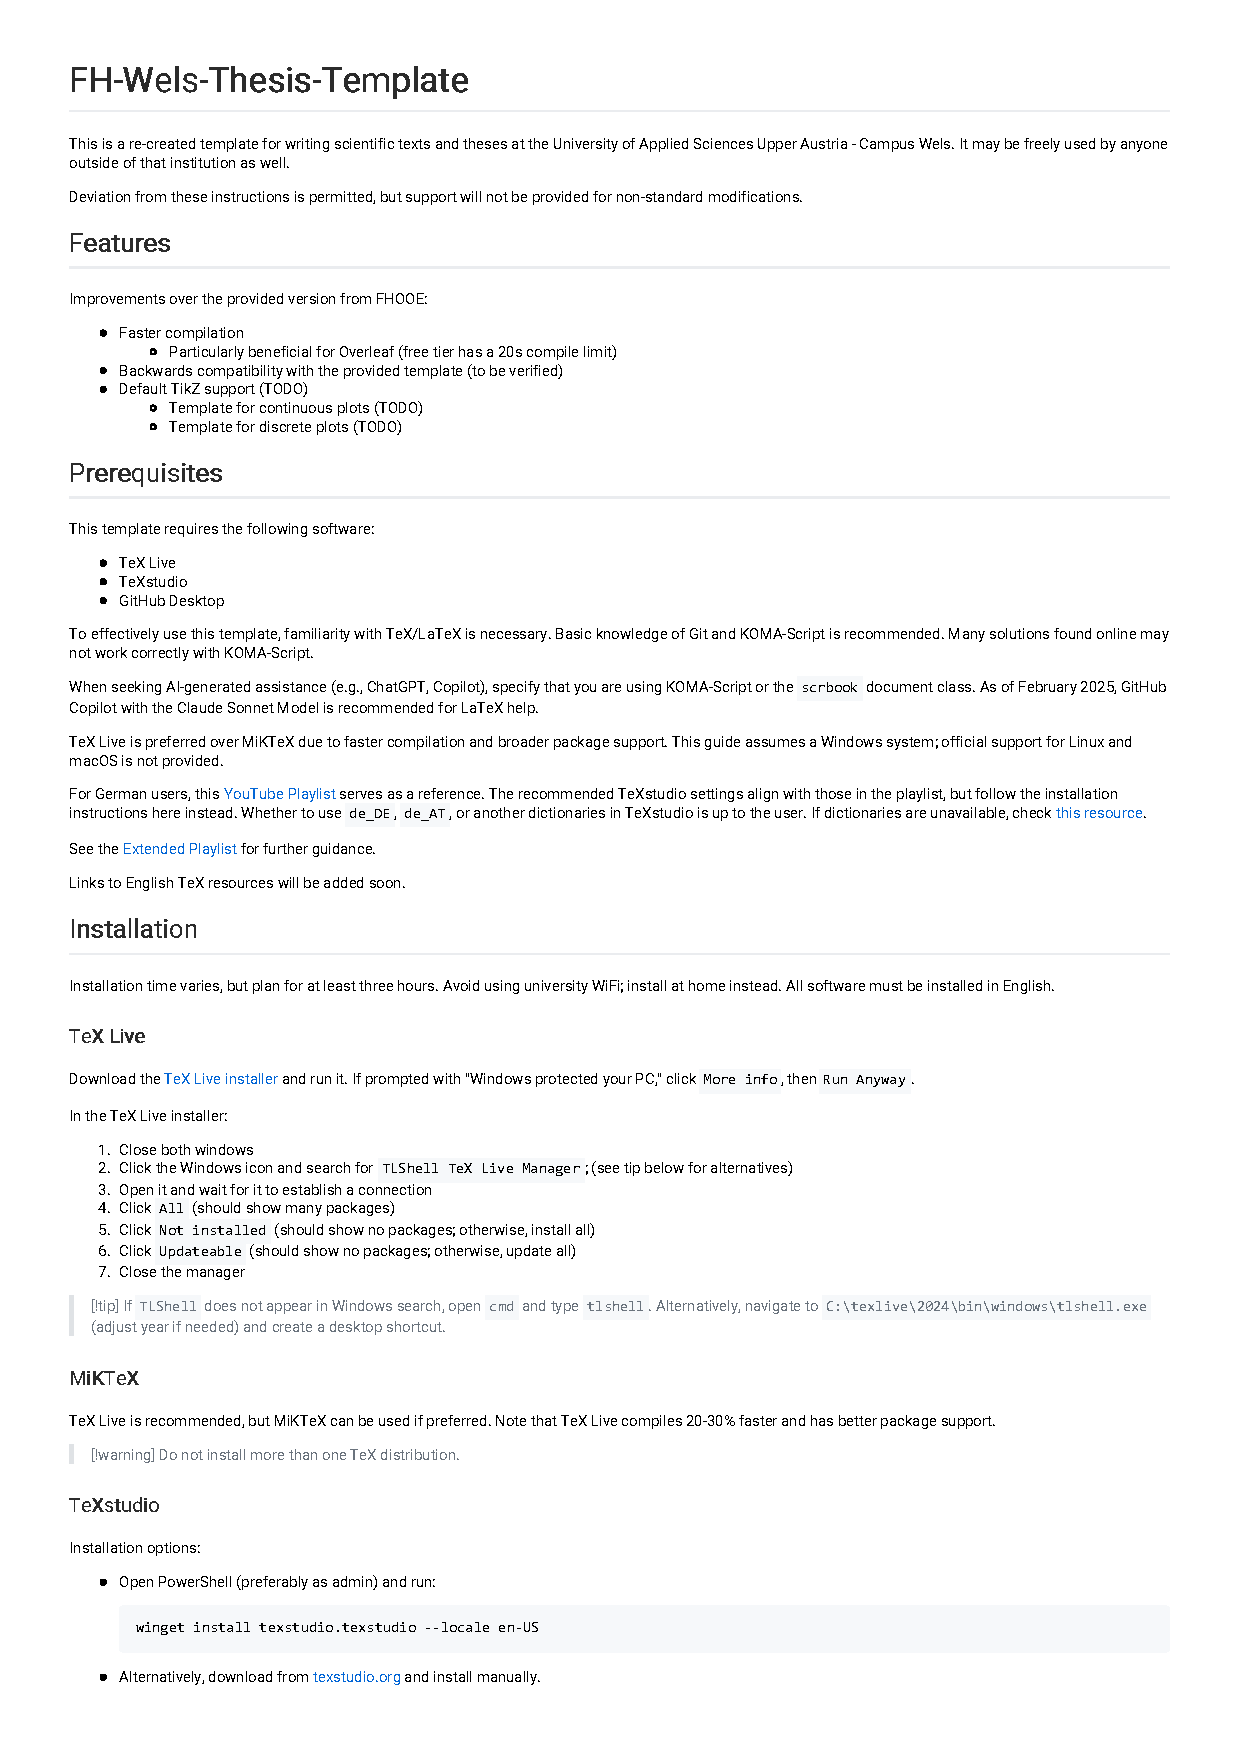
\includepdf[pages=-,scale=0.7]{documents/README.pdf}
     % TODO [USER:demo]
        \chapter{Source Code}

Please be aware that the indentations in this code will be visible in the compiled PDF. Many styles are predefined for you, change them in \texttt{preamble/code.tex} if needed.

\section{Markup and data languages}
\subsection{\LaTeX{} code example}
\begin{lstlisting}[style=latexstyle]
\documentclass[
    oneside,
    bibliography=totocnumbered, % Include bibliography in TOC with number
    listof=totocnumbered,       % Include List of Tables/Figures in TOC with number
    numbers=noenddot            % Changes heading numbering from 1.1. to 1.1
    % appendixprefix = true     % Makes Appendix A... First appendix chapter, disable for one appendix
]{scrbook}
%%%%%%%%%%%%%%%%%%%%%%%%%%%%%%%%%%%%%%%%%%%%
\begin{document}
    Hello, world!

    \begin{equation}
        \pdv{\psi}{t}
        =
        \frac{\partial \psi}{\partial t}
    \end{equation}

\end{document}
\end{lstlisting}



\subsection{YAML code example}
You can also directly input the code of a file into the \verb|lstlisting| command.

\lstinputlisting[style=yamlstyle]{code/docker-compose.yaml}

\section{Programming languages}
\subsection{Python code example}
\begin{lstlisting}[style=pythonstyle]
def fibonacci(n):
    a, b = 0, 1
    while a < n:
        print(a, end=" ")
        a, b = b, a + b
    print()

# Example usage
fibonacci(50)

\end{lstlisting}

\subsection{Matlab code example}
\begin{lstlisting}[style=matlabstyle]
function fibonacci(n)
    a = 0;
    b = 1;
    while a < n
        fprintf('%d ', a);
        temp = a + b;
        a = b;
        b = temp;
    end
    fprintf('\n');
end

% Example usage
fibonacci(50)
\end{lstlisting}


\subsection{Wolfram Mathematica code example}
\begin{lstlisting}[style=wolframstyle]
FibonacciSequence[n_] := Module[{a = 0, b = 1, temp},
    While[a < n,
        Print[a, " "];
        temp = a + b;
        a = b;
        b = temp;
    ]
]

(* Example usage *)
FibonacciSequence[50]

\end{lstlisting}


\subsection{C code example}
\begin{lstlisting}[style=cstyle]
#include <stdio.h>

void fibonacci(int n) {
    int a = 0, b = 1, temp;
    while (a < n) {
        printf("%d ", a);
        temp = a + b;
        a = b;
        b = temp;
    }
    printf("\n");
}

int main() {
    fibonacci(50);
    return 0;
}
\end{lstlisting}




%---------------------------------------------------------------------------%
\clearpage
\subsection{Longer code example (C)}

The following is the main.cpp from the TeXstudio GitHub repository. Direct Link:

https://github.com/texstudio-org/texstudio/blob/master/src/main.cpp

\begin{lstlisting}[style=cstyle]
/***************************************************************************
*   copyright       : (C) 2003-2007 by Pascal Brachet                     *
*   addons by Frederic Devernay <frederic.devernay@m4x.org>               *
*   addons by Luis Silvestre                                              *
*   http://www.xm1math.net/texmaker/                                      *
*                                                                         *
*   This program is free software; you can redistribute it and/or modify  *
*   it under the terms of the GNU General Public License as published by  *
*   the Free Software Foundation; either version 2 of the License, or     *
*   (at your option) any later version.                                   *
*                                                                         *
***************************************************************************/

#include "mostQtHeaders.h"
/*! \mainpage TexStudio
*
* \see Texstudio
* \see PDFDocument
*/

#include "texstudio.h"
#include "smallUsefulFunctions.h"
#include "debughelper.h"
#include "debuglogger.h"
#include "utilsVersion.h"
#include <qtsingleapplication.h>
#include <QSplashScreen>

#ifdef Q_OS_WIN32
#include "windows.h"
typedef BOOL (WINAPI *AllowSetForegroundWindowFunc)(DWORD);
#endif

class TexstudioApp : public QtSingleApplication
{
	public:
	bool initialized;
	QString delayedFileLoad;
	Texstudio *mw;  // Moved from private:
	TexstudioApp(int &argc, char **argv);
	TexstudioApp(QString &id, int &argc, char **argv);
	~TexstudioApp();
	void init(QStringList &cmdLine);   // This function does all the initialization instead of the constructor.
	/*bool notify(QObject* obj, QEvent* event){
		//really slow global event logging:
		//qWarning(qPrintable(QString("%1 obj %2 named %3 typed %4 child of %5 received %6").arg(QTime::currentTime().toString("HH:mm:ss:zzz")).arg((long)obj,8,16).arg(obj->objectName()).arg(obj->metaObject()->className()).arg(obj->parent()?obj->parent()->metaObject()->className():"").arg(event->type())));
		try {
			return QApplication::notify(obj,event);
		} catch (const std::exception& e){
			qDebug() << "Catched exception: " << e.what();
			return false;
		}
	}*/


	protected:
	bool event(QEvent *event);
};

TexstudioApp::TexstudioApp(int &argc, char **argv) : QtSingleApplication(argc, argv)
{
	mw = nullptr;
	initialized = false;
}

TexstudioApp::TexstudioApp(QString &id, int &argc, char **argv) : QtSingleApplication(id, argc, argv)
{
	mw = nullptr;
	initialized = false;
}

void TexstudioApp::init(QStringList &cmdLine)
{
	QPixmap pixmap(":/images/splash.png");
	QSplashScreen *splash = new QSplashScreen(pixmap);
	splash->show();
	processEvents();

	mw = new Texstudio(nullptr, Qt::WindowFlags(), splash);
	connect(this, SIGNAL(lastWindowClosed()), this, SLOT(quit()));
	splash->finish(mw);
	delete splash;

	initialized = true;

	if (!delayedFileLoad.isEmpty()) cmdLine << delayedFileLoad;
	mw->executeCommandLine(cmdLine, true);
	if(!cmdLine.contains("--auto-tests")){
		mw->startupCompleted();
	}
}

TexstudioApp::~TexstudioApp()
{
	delete mw;
}

bool TexstudioApp::event(QEvent *event)
{
	if (event->type() == QEvent::FileOpen) {
		QFileOpenEvent *oe = static_cast<QFileOpenEvent *>(event);
		if (initialized) mw->load(oe->file());
		else delayedFileLoad = oe->file();
		event->accept();
		return true;
	}
	return QApplication::event(event);
}

QString generateAppId()
{
	QProcessEnvironment env = QProcessEnvironment::systemEnvironment();
	QString user = env.value("USER");
	if (user.isEmpty()) {
		user = env.value("USERNAME");
	}
	return QString("%1_%2").arg(TEXSTUDIO,user);
}

QStringList parseArguments(const QStringList &args, bool &outStartAlways)
{
	QStringList cmdLine;
	for (int i = 1; i < args.count(); ++i) {
		QString cmdArgument =  args[i];

		if (cmdArgument.startsWith('-')) {
			// various commands
			if (cmdArgument == "--start-always")
			outStartAlways = true;
			else if (cmdArgument == "--no-session")
			ConfigManager::dontRestoreSession = true;
			else if ((cmdArgument == "-line" || cmdArgument == "--line") && (++i < args.count()))
			cmdLine << "--line" << args[i];
			else if ((cmdArgument == "-page" || cmdArgument == "--page") && (++i < args.count()))
			cmdLine << "--page" << args[i];
			else if ((cmdArgument == "-insert-cite" || cmdArgument == "--insert-cite") && (++i < args.count()))
			cmdLine << "--insert-cite" << args[i];
			else if (cmdArgument == "--ini-file" && (++i < args.count())) {
				// deprecated: use --config instead
				ConfigManager::configDirOverride = QFileInfo(args[i]).absolutePath();
			}
			else if (cmdArgument == "--config" && (++i < args.count()))
			ConfigManager::configDirOverride = args[i];
			#ifdef DEBUG_LOGGER
			else if ((cmdArgument == "--debug-logfile") && (++i < args.count()))
			debugLoggerStart(args[i]);
			#endif
			else
			cmdLine << cmdArgument;
		} else {
			if(cmdArgument.endsWith(".txss")||cmdArgument.endsWith(".txss2")){
				// explicit session restor
				// disable restoring of last session
				ConfigManager::dontRestoreSession = true;
			}
			cmdLine << QFileInfo(cmdArgument).absoluteFilePath();
		}
	}
	return cmdLine;
}

bool handleCommandLineOnly(const QStringList &cmdLine) {
	// note: stdout is not supported for Win GUI applications. Will simply not output anything there.
	if (cmdLine.contains("--help")) {
		QTextStream(stdout) << "Usage: texstudio [options] [file]\n"
		<< "\n"
		<< "Options:\n"
		<< "  --config DIR              use the specified settings directory\n"
		<< "  --master                  define the document as explicit root document\n"
		<< "  --line LINE[:COL]         position the cursor at line LINE and column COL\n"
		<< "  --insert-cite CITATION    inserts the given citation\n"
		<< "  --start-always            start a new instance, even if TXS is already running\n"
		<< "  --pdf-viewer-only         run as a standalone pdf viewer without an editor\n"
		<< "  --page PAGENUM            display a certain page in the pdf viewer\n"
		<< "  --no-session              do not load/save the session at startup/close\n"
		<< "  --texpath PATH            force resetting command defaults with PATH as first search path\n"
		<< "  --version                 show version number\n"
		#ifdef DEBUG_LOGGER
		<< "  --debug-logfile pathname  write debug messages to pathname\n"
		#endif
		;
		return true;
	}

	if (cmdLine.contains("--version")) {
		QTextStream(stdout) << "TeXstudio " << TXSVERSION << " (" << TEXSTUDIO_GIT_REVISION << ")\n";
		return true;
	}

	return false;
}

int main(int argc, char **argv)
{
	QString appId = generateAppId();
	#if QT_VERSION >= QT_VERSION_CHECK(5,6,0)
	if(qEnvironmentVariableIntValue("TEXSTUDIO_HIDPI_SCALE")>0){
		QApplication::setAttribute(Qt::AA_EnableHighDpiScaling);
	} else {
		QApplication::setAttribute(Qt::AA_DisableHighDpiScaling);
	}
	#endif
	// This is a dummy constructor so that the programs loads fast.
	TexstudioApp a(appId, argc, argv);
	bool startAlways = false;
	QStringList cmdLine = parseArguments(QCoreApplication::arguments(), startAlways);

	if (handleCommandLineOnly(cmdLine)) {
		return 0;
	}

	if (!startAlways) {
		if (a.isRunning()) {
			#ifdef Q_OS_WIN32
			AllowSetForegroundWindowFunc asfw = (AllowSetForegroundWindowFunc) GetProcAddress(GetModuleHandleA("user32.dll"), "AllowSetForegroundWindow");
			if (asfw) asfw(/*ASFW_ANY*/(DWORD)(-1));
			#endif
			a.sendMessage(cmdLine.join("#!#"));
			return 0;
		}
	}

	a.setApplicationName( TEXSTUDIO );
	#if (QT_VERSION >= QT_VERSION_CHECK(5, 7, 0)) && defined(Q_OS_LINUX)
	a.setDesktopFileName("texstudio");
	#endif
	a.init(cmdLine); // Initialization takes place only if there is no other instance running.

	QObject::connect(&a, SIGNAL(messageReceived(const QString&)),
	a.mw, SLOT(onOtherInstanceMessage(const QString&)));

	try {
		int execResult = a.exec();
		#ifdef DEBUG_LOGGER
		if (debugLoggerIsLogging()) {
			debugLoggerStop();
		}
		#endif
		return execResult;
	} catch (...) {
		#ifndef NO_CRASH_HANDLER
		catchUnhandledException();
		#endif
		throw;
	}
}
\end{lstlisting}    % TODO [USER:demo]

%===============================================================================%
\end{document}